% =============================================================================
% Manuscript: Quantum Agrivoltaic Digital Twin: Coordinated Vibronic Light-Harvesting,
%             Spectral Co-Design, Multifunctional Net Energy Benefit, and Quantum-Secured Telemetry
% Target: Applied Energy (Elsevier)
% Date:    September 23, 2026 (Applied Energy submission package)
% Authors: Teguia Kouam S.C., Goumai Vedekoi T., Tchapet Njafa J.-P.,
%          Nguenang J.-P., Nana Engo S.G.
% Note: submission package copied from Submission_Package_Nature_Energy_Manuscript;
%       base files preserved as *_BASE.pdf. Converted to elsarticle (preprint).

\documentclass[preprint,12pt]{elsarticle}
\usepackage[utf8]{inputenc}
\usepackage[T1]{fontenc}
\usepackage{amsmath,amssymb,amsfonts}
\usepackage{graphicx}
\graphicspath{{figures/}}
\usepackage{booktabs}
\usepackage{siunitx}
\usepackage{physics}
% mhchem v4 for chemical formulas (\ce{Pb^{2+}}, \ce{CO2}, etc.)
\usepackage[version=4]{mhchem}
% siunitx v3 ↔ physics compatibility: physics defines \qty, siunitx v3 redefines it.
% This shim ensures siunitx's \qty takes precedence at begin-document time.
\AtBeginDocument{\RenewCommandCopy\qty\SI}
\usepackage{xcolor}
\usepackage[colorlinks=true,linkcolor=blue,citecolor=blue,urlcolor=blue]{hyperref}
\usepackage[capitalise,nameinlink]{cleveref}
\usepackage{xr}
\externaldocument{AppliedEnergy_SM_2609}
% (elsarticle manages page geometry; the geometry package is intentionally not loaded)
\usepackage{lineno}

% ---- siunitx v3 configuration ----
\sisetup{
    locale = US,
    detect-all = true,
    group-minimum-digits = 4,
    separate-uncertainty = true,
    multi-part-units = single,
    range-phrase = {--},
    range-units = single,
    number-unit-product = \,,
    allow-number-unit-breaks = true,
}
\DeclareSIUnit{\yr}{yr}
\DeclareSIUnit{\USD}{USD}
\DeclareSIUnit{\tonne}{t}
\DeclareSIUnit{\ha}{ha}
\DeclareSIUnit{\hectare}{ha}
\DeclareSIUnit{\MWh}{MWh}
\DeclareSIUnit{\kWh}{kWh}
\DeclareSIUnit{\cubed}{^{3}}
\DeclareSIUnit{\m}{\meter}

% ---- Line numbering for review ----
\linenumbers
% ponytail: global stretch absorbs dense \qty chunks; tables narrowed individually
\emergencystretch=2.5em

\newcommand{\eqphift}{\Cref{eq:phi_ft}}

\begin{document}
% ponytail: lineno + frontmatter footnote insert = spurious overfull vbox at
% page-1 shipout; review numbering starts after the frontmatter (standard).
\nolinenumbers

\begin{frontmatter}

\title{Quantum-Enhanced Agrivoltaic Digital Twin: Spectral Co-Design, Multifunctional Net Energy Benefit, and Quantum-Secured Telemetry}

\author[udla]{Steve Cabrel Teguia Kouam\corref{cor1}}
\author[uy1]{Theodore Goumai Vedekoi}
\author[uy1]{Jean-Pierre Tchapet Njafa}
\author[udla]{Jean-Pierre Nguenang}
\author[uy1]{Serge Guy Nana Engo}

\cortext[cor1]{Corresponding author. Email: steve.teguia@facsciences-uy1.cm}

\address[udla]{Department of Physics, Faculty of Science, University of Douala, Cameroon}
\address[uy1]{Department of Physics, Faculty of Science, University of Yaound\'{e} I, Cameroon}
% TODO(author, F11): attach \orcid{...} identifiers to the \author entries above before upload.

\begin{abstract}
Agrivoltaic deployment is constrained by a system-level trade-off: static semi-transparent photovoltaic modules resolve the food--energy land conflict only by uniformly sacrificing either electrical output or crop productivity. Here we present a quantum-guided agrivoltaic system in which a semi-transparent organic photovoltaic layer couples to a plasmonic nanoparticle-on-mirror (NPoM) cavity acting as an active spectral shaper. By transmitting narrow bands at \qtylist{750;820}{\nm}, the system prepares polaron-dressed states in the Fenna--Matthews--Olson photosynthetic complex, extending exciton coherence by \qty{50}{\percent} and achieving an area-weighted global canopy yield of \qty{97.1}{\percent}. The NPoM sentinel layer enables multiplexed SERS and quantum dot diagnostics of agricultural contaminants and crop stress. On the macroscopic scale, the shield reduces crop evapotranspiration by \qty{28}{\percent} and yields a Net Ecological Benefit of \qty{72.6}{\kg\of{\ce{CO2e}}\per\m\squared\per\yr}. A BB84 quantum link secures the IoT telemetry. Finally, techno-economic analysis of a Cameroonian micro-module gives a payback period of \qty{4.32}{\yr}, identifying conditions under which the multifunctional net benefit stays positive for the modeled \qty{500}{\m\squared} cooperative case.
\end{abstract}

\begin{keyword}
quantum agrivoltaics \sep FMO complex \sep vibronic coherence \sep plasmonic nanoparticle-on-mirror cavity \sep SERS diagnostics \sep FAO-56 evapotranspiration \sep agrivoltaic techno-economics
\end{keyword}

\end{frontmatter}
% ponytail: frontmatter (title + 6 authors + 3 addresses + abstract + keywords)
% overshoots textheight by ~29pt; give page 1 two extra lines instead of
% reflowing approved frontmatter content.
\enlargethispage{32pt}
\linenumbers

% =============================================================================
% INTRODUCTION
% =============================================================================

\section{Introduction}

Agrivoltaics co-locates photovoltaic (PV) systems and agricultural cultivation to mitigate the land-use competition between food production and renewable energy generation~\cite{Goetzberger1981,Dupraz2011}. Land-use optimization and mobile-PV foundations for this field were established in \textit{Applied Energy}~\cite{Valle2017,Amaducci2018}. Recent syntheses systematize overhead, vertical, and tracking typologies with land-equivalent-ratio and levelized-cost metrics~\cite{Mahim2025}.
Across these studies, three gaps recur and remain unresolved.
The optical architecture is \emph{static}: semi-transparent PV claddings act as fixed spectral filters that attenuate irradiance uniformly, trading electrical output for crop biomass without optimization of the spectral light-sharing window~\cite{Thompson2020,Zhao2023}. Dynamic, physics-guided spectral management has not been transposed into an operating agrivoltaic stack. The cost of stasis is quantifiable: in the mode-volume scan reported below, the forward transfer yield varies by a factor of 1.6 and the SERS enhancement by a factor of 48 across the accessible range (\Cref{tab:npom_volume_scan}), so a statically chosen cladding fixes the energy--diagnostics balance at deployment with no ability to re-trade it. The scan probes the strong-coupling penalty only: all seven volumes carry the NPoM channel, and the filtered-excitation gains quantified next apply to the NPoM-free fraction at every point of the scan.
Techno-economic and lifecycle assessments remain decoupled from the underlying device physics: electricity, crop, water, and carbon accounts are evaluated subsystem by subsystem, so multifunctional trade-offs are described rather than co-optimized~\cite{Ravilla2024,Bellone2024}. The cost of this decoupling is concrete: accounting that ignores the local transport physics would credit the canopy with the passive baseline of \num{0.980} instead of the physically consistent \num{0.971} --- and would never discover that the \qty{91.8}{\percent} local penalty costs only 0.9 points globally, a stabilizing margin that makes NPoM integration viable.
The PV layer is likewise treated purely as an energy harvester: in-situ crop-stress and contaminant sensing is bolted on as separate hardware rather than co-designed with the optical stack, despite the maturity of field-deployable SERS analysis~\cite{CiallaMay2024}, of quantum-enabled agricultural workflows~\cite{Pook2025}, and of quantum-sensing readiness for precision agriculture~\cite{KaurJeet2026}. Co-design changes the economics of the sensing function: reusing the NPoM optical infrastructure delivers SERS diagnostics at a canopy-area cost of \qty{1}{\percent} and a canopy-yield cost of \qty{0.9}{\percent} relative to the passive baseline (\num{0.980} to \num{0.971}), instead of separate sensing hardware with its own capital and footprint.

The photosynthetic apparatus of green plants and bacteria has evolved under a spectrally structured photon flux, where specific wavelengths drive charge separation while others dissipate as heat~\cite{Blankenship2011}.
This spectral specificity lets the PV layer transmit only the photosynthetically active wavelengths while absorbing the remainder, converting the food-energy conflict into a problem of spectral co-design.

The Fenna--Matthews--Olson (FMO) complex of green sulfur bacteria serves as the model system for spectral light-sharing~\cite{Fenna1974}.
Its seven bacteriochlorophyll $a$ sites have been extensively characterized through two-dimensional electronic spectroscopy, revealing oscillatory coherence signatures that persist for hundreds of femtoseconds at cryogenic~\cite{Engel2007} and room temperature~\cite{Panitchayangkoon2010}.
Although the functional relevance of these quantum beats remains debated, consensus has emerged that vibronic coupling --- the hybridization of electronic transitions with underdamped protein vibrations --- governs the flow of excitation energy~\cite{Chin2013,Christensson2012}.
Non-Markovian frameworks such as the hierarchical equations of motion~\cite{Tanimura1989} and the process tensor hierarchy of pure states (PT-HOPS)~\cite{Varvelo2021,Citty2024} capture these effects with demonstrated numerical convergence. Device-adjacent uses of exact open-quantum-system methods remain rare: the closest precedent is a general HEOM library applied to light-harvesting and control problems without a photovoltaic product~\cite{Lambert2023}. Photonic-quantum solar design and vibronic-screening workflows likewise stop short of an operating device~\cite{LiuFang2026,Motlagh2024}.

Previous work demonstrated that spectral filtering of the excitation pulse --- aligning its spectrum with underdamped vibronic resonances at \qty{750}{\nm} and \qty{820}{\nm} --- extends coherence lifetimes by \qty{20}{\percent} to \qty{50}{\percent} in the 7-site FMO complex~\cite{TeguiaKouam2026}.
This selective vibronic excitation prepares polaron-dressed states that decouple from the dissipative protein-solvent bath. That companion paper, published in the \textit{Journal of Physical Chemistry Letters}, reports the analysis of the filter, the excitation-transport rate, and the single-pass conversion efficiency~\cite{TeguiaKouam2026}; the present work adds the 8-site trapping model, the monolithic OPV--NPoM hardware concept, the SERS field calibration, and the Net Ecological Benefit and lifecycle assessment developed below.
Single-photon experiments have confirmed that quantum coherence persists in individual light-harvesting complexes under ambient conditions~\cite{Li2023}, and quantum phase synchronization via exciton-vibrational energy dissipation has been identified as a mechanism sustaining long-lived coherence~\cite{Zhu2024}.
Here we extend this principle in three directions.

First, we introduce an 8-site FMO model with a non-Hermitian reaction center trap on sites 3 and 4, enabling quantitative computation of the forward transfer yield $\Phi_{\mathrm{FT}}$ as the time-integrated population captured by the reaction center.
Second, we embed the FMO complex in a nanoparticle-on-mirror (NPoM) plasmonic cavity~\cite{Chikkaraddy2016} that couples the biological light-harvesting system to the organic photovoltaic (OPV) layer through strong coherent coupling, forming a $9\times 9$ dressed Hamiltonian.
Third, we incorporate dynamic photo-protection mechanisms --- Floquet Stark detuning and flux-dependent optical limiting --- that mimic the non-photochemical quenching used by plants under high light stress.

We map this microscopic optimization onto a field-scale lifecycle assessment.
We parameterize crop evapotranspiration using the FAO-56 Penman--Monteith model~\cite{Allen1998} under the spectrally selective OPV shield, compute the Net Ecological Benefit (NEB) across three scenarios, and evaluate socioeconomic access through cooperative ownership models and BB84 quantum key distribution~\cite{Bennett1984} for secure IoT telemetry.
This multi-scale perspective~\cite{Vandamme2025} links angstrom-scale vibronic couplings to square-meter canopy yields, providing a unified modeling framework for quantum-guided agrivoltaics (\cref{fig:system_setup}).

The central question of this work is falsifiable: \emph{does an agrivoltaic stack whose spectral architecture is co-designed by exact non-Markovian quantum dynamics deliver a positive multifunctional net energy benefit (power $+$ crop $+$ water $+$ sensing) under field constraints, and which deployment barriers are physical rather than economic?}
Three subordinate questions structure the Results. (Q1) Device asks what the NPoM co-design costs and where the cost lands, quantified by the mode-volume scan (\Cref{tab:npom_volume_scan}) and located by the canopy-integration analysis. (Q2) Physics asks which microscopic states carry the trade-off: exact PT-HOPS dynamics localize the loss channels, and Floquet--Stark detuning with flux-dependent optical limiting tests whether they can be managed dynamically. (Q3) System asks whether the stack pays for itself, once coupled FAO-56 microclimate, cooperative techno-economics, and BB84-secured telemetry internalize every function into a single Net Ecological Benefit account.
Three falsifiable claims anchor the answer. The first, (F1) Microscopic, is that dual-band spectral filtering at \qty{750}{\nm} and \qty{820}{\nm} prepares polaron-dressed states that extend exciton coherence by \qty{50}{\percent} and raise the forward transfer yield by \qty{25}{\percent} at \qty{295}{\kelvin}.
The second, (F2) Device, is that confining the NPoM cavity to a \qty{1}{\percent} sentinel fraction preserves \qty{97.1}{\percent} of the global canopy trapping yield ($\Phi_{\mathrm{FT}}^{\mathrm{global}} = 0.971$) while retaining single-complex SERS diagnostics, despite the $>\qty{90}{\percent}$ local transport penalty quantified across the mode-volume scan.
The third, (F3) System, is that the FAO-56 smart shield cuts evapotranspiration by \qty{28}{\percent} ($\pm\qty{10}{\percent}$ microclimate uncertainty) and, combined with OPV generation and cooperative economics, yields a Net Ecological Benefit of \qty{72.6}{\kg\of{\ce{CO2e}}\per\m\squared\per\yr} and a \qty{4.32}{\yr} payback at \qty{30}{\percent} subsidy for the modeled \qty{500}{\m\squared} cooperative case.
We answer affirmatively but conditionally: the bounds (single-exciton treatment, site-independent baths, modeled fouling and matrix penalties, $\pm\qty{10}{\percent}$ microclimate band) are stated explicitly in the Limitations section of the Discussion.
The headline outcome, pictured in \Cref{fig:flat_canopy}, compresses this answer to one sentence: a \qty{91.8}{\percent} local transport penalty confined to a \qty{1}{\percent} sentinel area costs 0.9 points of canopy-scale trapping yield (\num{0.980} to \num{0.971}) while adding single-complex SERS diagnostics to the same footprint.
To keep a stack of this breadth auditable, each layer --- quantum dynamics, microclimate, economics, and security --- is validated separately in the Supporting Information (\Cref{SI-sec:convergence}--\Cref{SI-sec:gqas}), and every headline number below is traceable to a single figure or table.

% =============================================================================
% RESULTS
% =============================================================================

\section{Results}

\subsection{8-Site FMO Hamiltonian with reaction center trap}

\begin{table*}[htbp]
\centering
\small\setlength{\tabcolsep}{4pt}
\caption{\textbf{8-site FMO site energies and key electronic couplings (\unit{\per\cm})}. The near-degenerate antenna pair (Sites~1--2) feeds the trap funnel (Sites~3--4) through the strongly coupled 4--5--6 backbone; Site~8 extends the antenna manifold with couplings an order of magnitude below $J_{12}$ (strongest link $J_{18} = \qty{21.0}{\per\cm}$), so the 7-site transport references carry over to the 8-site network. These couplings set the transport timescale that the spectral filter exploits. Full coupling matrix (28 unique pairs) provided in \Cref{SI-sec:hamiltonian}.}
\label{tab:fmo_parameters}
\begin{tabular}{l *{8}{S[table-format=-2.1]} }
\toprule
\textbf{Parameter} & {\textbf{Site 1}} & {\textbf{Site 2}} & {\textbf{Site 3}} & {\textbf{Site 4}} & {\textbf{Site 5}} & {\textbf{Site 6}} & {\textbf{Site 7}} & {\textbf{Site 8}} \\
\midrule
$\varepsilon_n$ & 280 & 420 & 0 & 110 & 270 & 500 & 310 & 200 \\
$J_{n,n+1}$ & {---} & -87.7 & 30.0 & -53.5 & -70.7 & 81.1 & 39.7 & 12.0 \\
\bottomrule
\end{tabular}
\end{table*}

We construct an 8-site model of the FMO complex, extending the standard 7-site framework~\cite{Adolphs2006} by including the eighth bacteriochlorophyll, which extends the antenna manifold above Site~3 ($\varepsilon_8 = \qty{200}{\per\cm}$ relative to Site 3) with couplings ranging from $|J_{38}| = \qty{0.6}{\per\cm}$ to $J_{18} = \qty{21.0}{\per\cm}$ --- an order of magnitude below the $J_{12}$ backbone.
The electronic Hamiltonian is:
\begin{equation}
\hat{H}_{\mathrm{FMO}} = \sum_{n=1}^{8} \varepsilon_n \dyad{n} + \sum_{n \neq m} J_{nm} \dyad{n}{m} - i\Gamma_{\mathrm{RC}} \sum_{j \in \{3,4\}} \dyad{j}{j},
\label{eq:fmo_hamiltonian}
\end{equation}
where $\varepsilon_n$ are the site energies (relative to Site 3), $J_{nm}$ are the inter-site electronic couplings (all 28 unique pairs defined in \Cref{SI-sec:hamiltonian}), and $\Gamma_{\mathrm{RC}} = \qty{0.15}{\per\fs}$ is the effective irreversible reaction-center trapping rate, corresponding to a capture time $\tau_{\mathrm{trap}} \approx \qty{6.7}{\fs}$. This capture time is short compared with the 1-ps propagation window, so near-complete capture (the \num{0.98} passive baseline) is dynamically accessible in \cref{eq:phi_ft}~\cite{Renger2003}.
The anti-Hermitian term $-i\Gamma_{\mathrm{RC}}$ on Sites 3 and 4 (physical indices; Python indices 2 and 3) models the irreversible charge separation at the reaction center.
We verify that all 28 inter-site couplings are finite and that the non-Hermiticity is confined to the trapping diagonal terms (\Cref{SI-sec:hamiltonian}).

\subsection{NPoM plasmonic strong coupling}

The OPV-FMO interface is mediated by a nanoparticle-on-mirror (NPoM) architecture~\cite{Chikkaraddy2016}, where a gold nanoparticle (diameter \qty{80}{\nm}) is separated from a gold mirror by a \qty{1}{\nm} graphene monolayer spacer.
The graphene barrier prevents Dexter-type electron transfer while maintaining electromagnetic field enhancement.
The NPoM cavity supports an intense localized surface plasmon mode that couples coherently to the FMO optical transitions and mediates the optical interface with the OPV layer.

The single-emitter coupling strength follows the cavity quantum electrodynamics scaling:
\begin{equation}
g_0 = g_{\mathrm{ref}} \sqrt{\frac{V_{\mathrm{ref}}}{V_{\mathrm{mode}}}},
\label{eq:coupling_scaling}
\end{equation}
with $g_{\mathrm{ref}} = \qty{120}{\per\cm}$ at $V_{\mathrm{ref}} = \qty{1}{\nm\cubed}$~\cite{Chikkaraddy2016}.
At the sub-nanometer mode volumes accessible in NPoM cavities ($V_{\mathrm{mode}} < \qty{1}{\nm\cubed}$), $g_0$ ranges from \qty{120}{\per\cm} to over \qty{300}{\per\cm}, and the collective coupling $g_{\mathrm{eff}} \sim \qty{2000}{\per\cm}$ places the system in the strong-coupling regime ($g_{\mathrm{eff}} > \kappa$, where $\kappa \approx \qty{800}{\per\cm}$ is the plasmon linewidth).
A numerical guardrail caps $g_0$ at \qty{1000}{\per\cm} when $V_{\mathrm{mode}} \to 0$ to prevent divergences.
Recent advances in quantum-tunnel-junction plasmonic sources have demonstrated that such sub-nanometer cavities can be self-illuminating, eliminating the need for bulky external optics~\cite{Lee2025}.

The dressed Hamiltonian expands to $9\times 9$:
\begin{equation}
\hat{H}_{\mathrm{dressed}} = 
\begin{pmatrix}
\hat{H}_{\mathrm{FMO}} & \hat{V}_{\mathrm{pl}} \\
\hat{V}_{\mathrm{pl}}^{\dagger} & \hbar\omega_{\mathrm{pl}}
\end{pmatrix},
\label{eq:dressed_hamiltonian}
\end{equation}
where the plasmon mode at frequency $\omega_{\mathrm{pl}} \approx \qty{12500}{\per\cm}$ couples to the primary optical antenna sites (BChl 1 and 6, indices 0 and 5) with strength $g_0$.
\Cref{fig:quantum_dynamics}a shows the energy level diagram.

\subsection{Non-Markovian quantum dynamics}

We propagate the 9-site dressed system using the PT-HOPS/SBD formalism with production parameters: hierarchy depth $L=8$, $K=2$ Matsubara terms, time step $\Delta t = \qty{0.2}{\fs}$, and $n=100$ disorder realizations ($\sigma = \qty{50}{\per\cm}$ static disorder)~\cite{Varvelo2021,Citty2024}.
The bath is modeled as a Drude--Lorentz overdamped component ($\lambda_D = \qty{35}{\per\cm}$, $\gamma_D = \qty{50}{\per\cm}$) plus 12 underdamped vibronic modes from the Kleinekath\"{o}fer/Coker parameterization.
Convergence is verified through hierarchy depth sweeps ($L=6,7,8$) and Matsubara truncation tests ($K=1,2,3$); the maximum relative error between $L=7$ and $L=8$ populations is $\num{3.1e-11}$, and between $K=2$ and $K=3$ is $\num{3.3e-5}$ (\Cref{SI-sec:convergence}). Our companion study details and validates the computational feasibility, scaling, and memory-aware scheduling of these high-order simulations~\cite{TeguiaKouam2026}.

\Cref{fig:quantum_dynamics}b shows the exciton population dynamics of the sentinel NPoM configuration ($V = \qty{1.2}{\nano\m\cubed}$, $n=20$): the plasmon mode loads within \qty{10}{\fs} and captures \qty{82}{\percent} of the excitation, and the reaction-center population saturates at the strongly suppressed value reported in \Cref{tab:npom_volume_scan}. The forward transfer yield quantifies this capture:
\begin{equation}
\Phi_{\mathrm{FT}} = \Gamma_{\mathrm{RC}} \int_0^{t_{\mathrm{max}}} \sum_{j \in \{3,4\}} P_j(t)\,dt,
\label{eq:phi_ft}
\end{equation}
where $P_j(t) = \rho_{jj}(t)$ are the site populations and $t_{\mathrm{max}} = \qty{1}{\ps}$.

Under dual-band filtering, $\Phi_{\mathrm{FT}} = 0.89(3)$, compared to $\Phi_{\mathrm{FT}} = 0.71(2)$ for broadband excitation --- a relative enhancement of \qty{25}{\percent} (\Cref{tab:SI_matsubara_convergence}; parenthetical uncertainties are 1 standard deviation over the $n=100$ disorder ensemble). These filtered- and broadband-excitation reference trajectories (bare FMO, no NPoM channel) are inherited unchanged from our companion study, which reports their full trajectory sets, computed on the seven-site network with an otherwise identical PT-HOPS/SBD protocol~\cite{TeguiaKouam2026}; the eighth site added here couples an order of magnitude below the $J_{12}$ backbone (strongest link $J_{18} = \qty{21.0}{\per\cm}$; weakest link into the trapping pair $J_{38} = \qty{0.6}{\per\cm}$), so we carry the references over unchanged. The 8-site no-NPoM reference $\Phi_{\mathrm{FT}} = 0.980$ is the assumed passive capture efficiency of the unimpeded network --- a model input representing near-complete charge separation, not a trajectory integral: within the 1-ps window the off-cavity integral does not saturate, because the trapping sites retain steady-state population (\Cref{SI-sec:comparative_hdf5}). These references characterize the \qty{99}{\percent} passive fraction of the canopy and are therefore independent of, and complementary to, the NPoM mode-volume scan below, which probes the strong-coupling penalty on the sentinel fraction.
The coherence lifetime $\tau_c$, defined as the $1/e$ decay time of the $l_1$-norm coherence $C_{l_1}(t) = \sum_{i\neq j} |\rho_{ij}(t)|$~\cite{Baumgratz2014}, extends from \qty{280(25)}{\fs} (broadband) to \qty{420(35)}{\fs} (filtered) --- a \qty{50}{\percent} increase that is causally linked to the yield gain. The extended coherence suppresses the pure-dephasing rate, lengthening the effective transport mean-free path and increasing the fraction of the excitation wavepacket that reaches the reaction center before decohering.
The mechanism is identical to that established for the 7-site system~\cite{TeguiaKouam2026}: the red passband is quasi-resonant with the trapping-site pair (sites~3/4 at \qty{12210}{\per\cm} and \qty{12320}{\per\cm}, i.e.\ \qty{819}{\nm} and \qty{812}{\nm}; the \qty{100}{\per\cm} passband is centred on site~3 and lies within \qty{75}{\per\cm} of site~4), so the manifold members that bridge those sites to the bright exciton --- the \qty{180}{\per\cm} Franck--Condon mode of site~4 and the \qty{280}{\per\cm} mode of site~3 --- are the dressed set. Removing them leaves a residual reorganization energy $\lambda_{\mathrm{res}}^{\mathrm{filt}} = \qty{110}{\per\cm}$ instead of the full-bath $\lambda_{\mathrm{res}} = \qty{127.6}{\per\cm}$ (\Cref{SI-sec:polaron}); because pure dephasing scales as $\lambda_{\mathrm{res}}^{-2}$, this predicts a $\times 1.34$ coherence extension, consistent with the computed $\times 1.50(18)$ (\qty{280}{\fs} $\to$ \qty{420}{\fs}) within the $1\sigma$ lifetime uncertainty. The blue passband lies between the \qty{720}{\per\cm} and \qty{1050}{\per\cm} manifold members and acts as a transparent control window, consistent with the companion band scan in which moving the blue edge from \qty{730}{\nm} to \qty{770}{\nm} left $\Phi_{\mathrm{FT}}$ unchanged.

\subsection{NPoM cavity volume dependence of exciton transport}

The nanoparticle-on-mirror cavity couples the FMO complex to the OPV active layer through the strong coherent interaction described above, yet the plasmonic mode also acts as an additional population decay channel competing with reaction-center trapping.
To quantify this trade-off, we perform a sensitivity scan of the NPoM mode volume $V_{\mathrm{mode}}$, which controls the single-emitter coupling strength via $g_0 \propto V_{\mathrm{mode}}^{-1/2}$ (\Cref{eq:coupling_scaling}).
Smaller mode volumes produce stronger plasmon--exciton coupling but also enhance the plasmon's role as a population sink, diverting excitation away from the reaction center.

\begin{table}[htbp]
\centering
\caption{\textbf{NPoM mode volume sensitivity of the forward transfer yield and SERS enhancement.}
Baseline (no NPoM): $\Phi_{\mathrm{FT}} = 0.98$. All NPoM runs with $L=8$, $K=2$, $\Delta t = \qty{0.2}{\fs}$, $t_{\mathrm{max}} = \qty{1}{\ps}$. The $V_{\mathrm{mode}} = \qty{1.2}{\nm\cubed}$ entry is validated with $n=20$ trajectories ($\Phi_{\mathrm{FT}} = \num{0.0799 \pm 0.0005}$); remaining table entries use $n=2$ (an additional $n=100$ run at $V_{\mathrm{mode}} = \qty{0.8}{\nm\cubed}$ is discussed in the text). SERS enhancement $\mathrm{EF}_{\mathrm{SERS}} \propto (Q/V_{\mathrm{mode}})^2$ via Purcell factor scaling, normalized to $\mathrm{EF}_{\mathrm{SERS}} = 10^2$ at $V_{\mathrm{mode}} = \qty{0.8}{\nm\cubed}$~\cite{Chikkaraddy2016}. An independent $n=20$ re-simulation of all seven volumes with the corrected production code reproduces every entry within $\pm 0.002$ ($V_{\mathrm{mode}} = \qtylist{0.8;1.2}{\nm\cubed}$ exactly), cross-validating the low-$n$ screening values.}
\label{tab:npom_volume_scan}
\begin{tabular}{S[table-format=1.1] S[table-format=1.4] S[table-format=-2.1] S[table-format=4.0]}
\toprule
{$V_{\mathrm{mode}}$ (\unit{\nm\cubed})} & {$\Phi_{\mathrm{FT}}$} & {$\Delta$ vs.\ baseline (\unit{\percent})} & {$\mathrm{EF}_{\mathrm{SERS}}$} \\
\midrule
0.2  & 0.0505 & -94.8 & 1600 \\
0.4  & 0.0605 & -93.8 & 400 \\
0.6  & 0.0727 & -92.6 & 180 \\
0.8  & 0.0768 & -92.2 & 100 \\
1.0  & 0.0793 & -91.9 & 64 \\
1.2  & 0.0799 & -91.8 & 44 \\
1.4  & 0.0791 & -91.9 & 33 \\
\bottomrule
\end{tabular}
\end{table}

\Cref{tab:npom_volume_scan} summarizes the forward transfer yield across seven mode volumes spanning the experimentally accessible sub-nanometer range~\cite{Chikkaraddy2016}.
The yield increases monotonically with mode volume, from $\Phi_{\mathrm{FT}} = 0.0505$ at $V_{\mathrm{mode}} = \qty{0.2}{\nm\cubed}$ to a maximum of $\Phi_{\mathrm{FT}} = 0.0799$ at $V_{\mathrm{mode}} = \qty{1.2}{\nm\cubed}$, with a slight decrease at $\qty{1.4}{\nm\cubed}$.
The trend is logarithmic, with diminishing returns above $\qty{1.0}{\nm\cubed}$: increasing the volume further recovers only \qty{1}{\percent} of the baseline yield.

The physical origin of this suppression is the strong-coupling-induced hybridization of excitonic and plasmonic states.
The dressed eigenstates acquire a finite plasmonic character, which decays via the fast plasmon relaxation pathway ($\kappa \approx \qty{800}{\per\cm}$, $Q \approx 15$) rather than populating the reaction center.
At $V_{\mathrm{mode}} = \qty{0.2}{\nm\cubed}$, where $g_0$ is largest, the plasmonic admixture in the lower polariton branch reaches $\sim \qty{15}{\percent}$, diverting a corresponding fraction of the excitation flux.
As $V_{\mathrm{mode}}$ increases, $g_0$ decreases, the polariton splitting narrows, and the excitonic character of the bright states is partially restored.

Despite the monotonic recovery, all NPoM-on yields remain suppressed by more than \qty{90}{\percent} relative to the pristine FMO baseline ($\Phi_{\mathrm{FT}} = 0.98$).
Hence, in the strong collective-coupling regime accessible to NPoM cavities ($g_{\mathrm{eff}} \sim \qty{2000}{\per\cm}$), the plasmonic decay pathway fundamentally limits the maximum achievable transport efficiency.
The SERS enhancement factor ($\sim 10^2$ at $V_{\mathrm{mode}} = \qty{0.8}{\nm\cubed}$) scales as $\mathrm{EF}_{\mathrm{SERS}} \propto (Q/V_{\mathrm{mode}})^2$, following the Purcell enhancement of the local field at both the excitation and emission wavelengths.
\Cref{tab:npom_volume_scan} includes the calculated SERS enhancement for each mode volume, revealing a four-order-of-magnitude range ($33$ to $1.6\times10^3$) across the scanned volumes. The optimal volume represents a compromise: $V_{\mathrm{mode}} \approx \qty{1.2}{\nm\cubed}$ maximizes transport yield ($\Phi_{\mathrm{FT}} = 0.0799$) while retaining SERS sensitivity ($\mathrm{EF}_{\mathrm{SERS}} \approx 44$).
The tabulated $\mathrm{EF}_{\mathrm{SERS}}$ values are a \emph{relative} Purcell scaling normalized to $10^2$ at $V_{\mathrm{mode}} = \qty{0.8}{\nm\cubed}$, not absolute single-molecule enhancements: absolute SERS in sub-nanometer NPoM gaps is measured at $10^6$ and above~\cite{Baumberg2019}, so single-complex detection of the \qty{180}{\per\cm} Franck--Condon mode remains within the demonstrated capability of this geometry~\cite{CiallaMay2024}. This compromise only works because of the sentinel architecture --- no volume on the scan simultaneously restores transport and maximizes diagnostics, which is precisely why the \qty{1}{\percent} area split, not a better volume, is the design lever.
By contrast, $V_{\mathrm{mode}} = \qty{0.2}{\nm\cubed}$ maximizes SERS sensitivity ($1.6\times10^3$) at the cost of the lowest transport yield ($\Phi_{\mathrm{FT}} = 0.0505$), a trade-off better suited to diagnostic-only applications where photochemical efficiency is secondary. At the reference volume, a dedicated $n=100$ production run at $V_{\mathrm{mode}} = \qty{0.8}{\nm\cubed}$ confirms the same limiting behavior ($\Phi_{\mathrm{FT}} = 0.0768$, final plasmon population \num{0.79}; \Cref{SI-sec:comparative_hdf5}).

Reducing the temperature to \qty{77}{\kelvin} (analyzed as a theoretical limit-case for thermal phonon suppression in \Cref{SI-sec:cryo}) doubles the trapping yield to $\Phi_{\mathrm{FT}} = 0.1685$. In the main agrivoltaic operating regime at \qty{295}{\kelvin}, the maximum trapped population on sites~3+4 remains at $\num{3.8e-3}$ for $V_{\mathrm{mode}} = \qty{1.2}{\nm\cubed}$, requiring the multi-scale sentinel fraction strategy to bypass plasmonic loading.

All room-temperature runs exhibit perfect trace conservation ($\Tr\rho = \num{1.0000 \pm 0.0000}$), validating the numerical stability of the PT-HOPS/SBD propagator. The $V=\qty{0.8}{\nm\cubed}$ configuration was run with $n=100$ disorder realizations; the $V=\qty{1.2}{\nm\cubed}$ configuration was validated with $n=20$ trajectories ($\Phi_{\mathrm{FT}} = 0.0799$, within \qty{0.6}{\percent} of the $n=2$ estimate of $0.0804$). The baseline NPoM-off run ($n=20$) is shown as a limiting-case reference; quantitative comparison across configurations is limited by the differing trajectory counts.

\subsection{Global canopy yield integration}

Because the NPoM SERS diagnostic mode suppresses local excitonic transport through plasmon population loading, it need only cover a \qty{1}{\percent} sentinel fraction $\alpha$ of the canopy area. The remaining \qty{99}{\percent} operates in passive OPV mode, preserving the near-baseline forward transfer yield $\Phi_{\mathrm{FT}}^{\mathrm{passive}} = 0.980$. The area-weighted \emph{global} canopy trapping yield is therefore:
\begin{equation}
  \Phi_{\mathrm{FT}}^{\mathrm{global}} = \alpha\,\Phi_{\mathrm{FT}}^{\mathrm{NPoM}} + (1-\alpha)\,\Phi_{\mathrm{FT}}^{\mathrm{passive}},
  \label{eq:phi_global}
\end{equation}
yielding $\Phi_{\mathrm{FT}}^{\mathrm{global}} = 0.971$ at $\alpha = 0.01$ and $\Phi_{\mathrm{FT}}^{\mathrm{NPoM}} = 0.080$ (or $0.0799$ precisely); device-level excitation transfer is thus maintained near baseline even though transport is suppressed locally on the sentinel.
$\Phi_{\mathrm{FT}}^{\mathrm{global}}$ is a device-level metric: crop productivity is governed by the photosynthetically active radiation transmitted through the module (the AVT/PAR budget), not by excitonic trapping in the FMO layer --- the two are optically coupled only through the shared passband design, which is why no coherence-derived gain is booked in the crop revenue.
Because \Cref{eq:phi_global} is linear in $\alpha$, the flatness of \Cref{fig:flat_canopy}b is an accounting identity rather than an independent dynamical result; what carries physical content are the two reference endpoints ($\num{0.080}$, measured on the sentinel run, and $\num{0.980}$, the passive capture-efficiency cap) that enter it.
The identity converts those endpoints into a design envelope: solving \Cref{eq:phi_global} for $\alpha$ gives a sentinel fraction of up to \qty{3.3}{\percent} before the global yield falls below $0.95$, and up to \qty{8.9}{\percent} before it falls below $0.90$.
The diagnostic area therefore has a factor $\sim 3$ of headroom over the \qty{1}{\percent} assumed here --- the co-design lever is not a better mode volume but how much area one is willing to spend on sensing.

\subsection{Dynamic photo-protection via Floquet--Stark detuning and flux-dependent optical limiting}

Under high solar flux ($> \qty{800}{\W\per\m\squared}$), the OPV dielectric constant changes dynamically, inducing a time-dependent Stark shift of the excitonic levels that detunes the OPV--FMO coupling.
We model this as a Floquet driving term:
\begin{equation}
\hat{H}_{\mathrm{Stark}}(t) = V_0 \cos(\omega_{\mathrm{F}} t) \left( \dyad{1}{1} + \dyad{6}{6} \right),
\label{eq:stark_detuning}
\end{equation}
with amplitude $V_0 = \qty{0.05}{\eV}$ and frequency $\omega_{\mathrm{F}} = \qty{1.2}{\THz}$.
Above threshold, the detuning shifts the OPV exciton energies out of resonance with the FMO absorption bands. With $V_0 = \qty{0.05}{\eV} = \qty{403}{\per\cm}$ --- $4.6\times$ the largest inter-site coupling $|J_{12}| = \qty{87.7}{\per\cm}$ --- the single-channel transmission factor of the resonant site-1 and site-6 pathways falls to $J^2/(J^2 + V_0^2) \approx 0.05$, i.e. these two antenna channels are effectively closed while the six alternative pathways through the network remain open (\Cref{fig:npq_switch}a). To prevent rapid, noise-induced oscillations under fluctuating cloud cover, we implement a hysteresis buffer of $\pm \qty{50}{\W\per\m\squared}$ (the detuning switch activates at \qty{850}{\W\per\m\squared} and deactivates only when the flux drops below \qty{750}{\W\per\m\squared}).

Concurrently, the NPoM cavity exhibits a flux-dependent optical-limiting response~\cite{Aspelmeyer2014} that suppresses transmission at the \qty{750}{\nm} and \qty{820}{\nm} channels under high flux --- the intensity-dependent counterpart of the optomechanical modulation of the picocavity resonance (we use ``optical limiting'' rather than ``transparency'' deliberately: the engineered observable here is a \emph{reduction} of passband transmission with flux).
The transmission is modulated as:
\begin{equation}
T_{\mathrm{OL}}(I) = T_0 \left(1 + \frac{I}{I_{\mathrm{sat}}}\right)^{-1},
\label{eq:omit}
\end{equation}
where $I$ is the incident flux and $I_{\mathrm{sat}} = \qty{800}{\W\per\m\squared}$.
At \qty{1000}{\W\per\m\squared}, the transmission drops to \qty{44}{\percent} of baseline (\Cref{fig:npq_switch}b), providing dynamic protection against exciton overload.
At zero flux (night mode), both mechanisms return to zero without singularities (\Cref{SI-sec:npq}).

\subsection{In situ SERS optomechanical diagnostics and environmental robustness}

The NPoM platform enables non-destructive readout of FMO vibrational states via surface-enhanced Raman scattering (SERS)~\cite{Langer2020}. Recent scoping reviews of in-situ agrivoltaic sensing list no SERS or plasmonic category~\cite{DiDomenico2026} --- the integration gap addressed here.
Multilayer graphene--metal plasmonic architectures have demonstrated detection sensitivities exceeding conventional SPR biosensors by an order of magnitude~\cite{Bahmani2026}.
The optomechanical coupling between the plasmon mode and FMO molecular vibrations ($g_{\mathrm{om}} = 0.01$) produces a SERS enhancement factor of $\mathrm{EF}_{\mathrm{SERS}} = 44$ at the optimal $V_{\mathrm{mode}} = \qty{1.2}{\nm\cubed}$, reaching $1.6\times10^{3}$ for the smallest scanned mode volumes.

Beyond the three canonical BChl $a$ vibrational modes previously identified (\qty{180}{\per\cm}, \qty{740}{\per\cm}, \qty{1145}{\per\cm}), we assign three spectroscopic target signatures to the sentinel sub-system, plus a fourth, non-spectroscopic readout handled by a separate NV-diamond microfluidic assay.
Oxidative stress is read out through the C--C stretch of conjugated chlorophyll $a$ at \qty{1145}{\per\cm}, with a detection limit of \qty{50}{\nano\mol\per\L} in the pre-necrotic regime~\cite{CiallaMay2024}.
Pesticide contamination by 2,4,5-trichlorophenoxyacetic acid (2,4,5-T) is detected via its characteristic Raman peak at \qty{1435}{\per\cm} (LOD = \qty{1}{\nano\mol\per\L} under controlled conditions), leveraging the plasmonic hot-spot amplification in the NPoM gap~\cite{CiallaMay2024}.
Heavy metal contamination of irrigation water (\ce{Pb^{2+}}) is quantified through Stern--Volmer fluorescence quenching of encapsulated \ce{CdTe/ZnSe} quantum dots sealed within the NPoM sensor-probe polymer matrix (LOD = \qty{31.8}{\nano\mol\per\L} under controlled conditions)~\cite{Mohammed2023}; unlike bare gold surfaces, the encapsulated probe is immune to dust and biofouling.
Cross-sensitivity between soil moisture and \ce{Pb^{2+}} contamination is resolved by dual spectral interrogation: heavy metals modify the Stern--Volmer quenching intensity and fluorescence decay time, whereas soil moisture alters the local dielectric constant, producing spectral broadening orthogonal to the metal-induced quenching signature.
Pathogen detection uses Nitrogen-Vacancy (NV) center nanodiamond sensors operated in a microfluidic ``Point-of-Care'' (Lab-on-a-Chip) desktop reader at the greenhouse hub (\cref{SI-sec:nv_diamond}). These solid-state quantum sensors detect paramagnetic bacterial metabolites from sap or irrigation water samples at pre-symptomatic stages (LOD = \qty{0.8}{\nano\mol\per\L} under controlled conditions; the agricultural matrix will degrade in-field sensitivity, a loss mitigated by the graphene barrier and \textit{DynamicCalibrator} corrections).

\Cref{fig:npq_switch}c shows the simulated Raman spectrum for the three BChl $a$ modes under active NPoM coupling.
The relative intensities encode the instantaneous exciton population distribution, providing a direct optical probe of the energy transfer pathway.

Environmental robustness under realistic agricultural conditions (dust, bird droppings, microbial fouling) is modeled at three infrastructure levels.
At the OPV panel level, the soiling factor $\eta_{\mathrm{soil}}(t)$ decays exponentially with days since last cleaning:
\begin{equation}
  \eta_{\mathrm{soil}}(t) = \max\!\left(1 - 0.005\,t_{\mathrm{days}},\; 0.75\right),
  \label{eq:soiling}
\end{equation}
which limits maximum OPV efficiency loss to \qty{25}{\percent} at the worst-case cleaning interval (reached after \qty{50}{\day}); the \qty{800}{\USD\per\yr} cleaning line of the cooperative OPEX corresponds to seven or eight interventions per year at $\sim$\qty{110}{\USD} each, i.e.\ a schedule that never reaches the floor.
At the sensor level, the graphene monolayer spacer of each NPoM cavity is functionalized with a zwitterionic polymer coating~\cite{Kumar2022,Do2025}, modeled in our simulations to preserve $\geq\qty{90}{\percent}$ quantum coherence after \qty{60}{\day} continuous field immersion; it is the primary anti-fouling barrier, physically repelling microbial adhesion and protein adsorption. A thin-film micro-shielding layer (\qty{1}{\micro\meter} to \qty{5}{\micro\meter} of \ce{SiO2} or \ce{Al2O3}) around the NPoM picocavity and CQD sensor tip further attenuates the diurnal temperature excursion at the quantum probe, reducing the thermal-drift contribution by the factor $(1-\eta_{\mathrm{shield}})$, with $\eta_{\mathrm{shield}} = 0.85$ (\cref{SI-sec:thermal_shielding}). The \textit{DynamicCalibrator} module --- an exponential moving average of daily reference readings ($\alpha = 0.1$) --- operates as a tertiary safety net: it applies a multiplicative correction factor and raises a drift alarm when the baseline shifts by more than \qty{20}{\percent}, at which point OPV panel cleaning is scheduled.

\subsection{Smart shield microclimate: FAO-56 evapotranspiration}

The spectrally selective OPV layer functions as a ``smart shield'' that blocks ultraviolet and near-infrared radiation while transmitting photosynthetically active bands. Passive solar-greenhouse heating with PV co-generation is an established precedent~\cite{Wu2023Energies}; the present shield differs by actively co-designing the transmitted spectrum against the vibronic resonances quantified above.
We parameterize the greenhouse microclimate using the FAO-56 Penman--Monteith equation~\cite{Allen1998} adapted for shaded conditions:
\begin{equation}
\mathrm{ET}_c = \frac{0.408 \Delta R_n + \gamma \frac{900}{T+273} u (e_s - e_a)}{\Delta + \gamma(1 + 0.34 u)} \, K_c,
\label{eq:fao56}
\end{equation}
where $R_n$ is the net radiation attenuated by the array-level OPV shading factor $f_{\mathrm{shade}} = 0.41$ (with soil heat flux $G \approx 0$ assumed for daily timescales under greenhouse shielding), $\Delta$ is the slope of the saturation vapor pressure curve, $\gamma$ is the psychrometric constant, $u$ is wind speed, $e_s - e_a$ is the vapor pressure deficit, and $K_c = 0.85$ is the crop coefficient. All annual water, carbon, and cash figures quoted in this work are produced by the annual FAO-56 and LCA accounting chain described in the Methods; the orchestrator's per-tick digital-twin water balance is an operational monitor on the same FAO-56 path, not an independent derivation.
The shading factor is not a free parameter: it is the product of the module's ground-coverage ratio and its complemented average visible transmittance, $f_{\mathrm{shade}} = \mathrm{GCR}\,(1-\tau_{\mathrm{AVT}}) = 0.55 \times 0.75 = 0.41$, so the canopy-level attenuation and the $\qty{15}{\percent}$/$\qty{25}{\percent}$ efficiency--transmittance module assumption (\Cref{sec:methods_poc}) describe the same stack.

Under standard conditions --- clear-sky reference day with $R_n = \qty{14.05}{\mega\joule\per\m\squared\per\day}$ (\num{0.677} of the \qty{5.76}{\kWh\per\m\squared\per\day} $=$ \qty{20.74}{\mega\joule\per\m\squared\per\day} daily horizontal irradiance after albedo and net longwave loss, consistent with a \qty{600}{\W\per\m\squared} midday peak), \qty{25}{\celsius}, \qty{60}{\percent} humidity, \qty{2}{\m\per\s} wind --- the open-field evapotranspiration is \qty{4.5}{\mm\per\day}.
With the OPV smart shield, $\mathrm{ET}_c$ drops to \qty{3.2}{\mm\per\day} --- a \qty{28}{\percent} reduction --- translating to \qty{1.26}{\mm\per\day}, i.e.\ \qty{460}{\L\per\m\squared\per\yr} when annualized over \qty{365}{\day} (\Cref{fig:lca_comparison}a).
The crop coefficient $K_c = 0.85$ accounts for the reduced transpiration demand under partial shade~\cite{Allen1998}.

\subsection{Socioeconomic viability and cooperative payback}

Socioeconomic analysis (\Cref{SI-sec:socioeconomic}) is rescaled to a \qty{500}{\m\squared} high-value floriculture micro-module (strawberries and cut flowers, \qty{4.5}{\USD\per\kg} at \qty{8.2}{\kg\per\m\squared\per\yr}), reducing the entry-level capital expenditure to \qty{161000}{\USD} (\qty{322}{\USD\per\m\squared}). Our \$/kWh accounting follows the Monte-Carlo techno-economic logic established for European agrivoltaic configurations~\cite{Zidane2025}.
A blended-finance subsidy of \qty{30}{\percent} reduces the net CAPEX to \qty{112700}{\USD}.

Three operating expenditure streams are modeled: extension services and technician training (\qty{1200}{\USD\per\yr}), OPV panel cleaning (\qty{800}{\USD\per\yr}), and general maintenance (\qty{2000}{\USD\per\yr}), for a total annual OPEX of \qty{4000}{\USD\per\yr}.
The net annual cash flow of \qty{26075}{\USD\per\yr} (from \qty{30075}{\USD\per\yr} total revenue minus \qty{4000}{\USD} of OPEX) yields a simple payback period of \qty{4.32}{\yr} (or \qty{6.17}{\yr} without subsidy) and a 10-year discounted NPV of $+$\qty{34630}{\USD} at a \qty{12}{\percent} risk-adjusted discount rate that we adopt as the Sub-Saharan infrastructure-finance assumption (\Cref{fig:lca_comparison}c). Holding other inputs fixed, varying the subsidized net CAPEX by $\pm\qty{20}{\percent}$ shifts the payback to \qtyrange{3.46}{5.18}{\yr}; a \qty{50}{\percent} higher OPEX (\qty{6000}{\USD\per\yr}) gives \qty{4.49}{\yr}, and \qty{20}{\percent} lower revenue gives \qty{5.61}{\yr}.
Beyond one-at-a-time variations, a seeded Monte Carlo ($10^5$ iterations, seed 42, the same engine as the in-pipeline uncertainty band) co-samples all inputs jointly: \qty{10}{\percent} each on excitation yield, generation, lifecycle footprint, CAPEX, and revenue, \qty{15}{\percent} on the water saving, and \qty{10}{\percent} on the grid emission factor. It returns NEB $= 72.6$ with a \qty{95}{\percent} interval of \qtyrange{54.3}{92.2}{\kg\of{\ce{CO2e}}\per\m\squared\per\yr}, a payback mean of \qty{4.38}{\yr} (the deterministic point estimate is \qty{4.32}{\yr}; the ratio estimator is slightly convex) with \qtyrange{3.36}{5.62}{\yr}, and an NPV mean of $+$\qty{34700}{\USD} with a \qty{95}{\percent} interval of \qtyrange{+700}{+68600}{\USD} --- the 5th-percentile NPV stays positive, so the investment case survives the joint input scatter, not only the single-factor sensitivities (\Cref{SI-sec:socioeconomic}).
A baseline CAPEX of \qty{322}{\per\m\squared} is a significant barrier in Sub-Saharan Africa relative to local income levels. Local construction materials (bamboo and timber framing instead of structural steel) and green chemical synthesis of gold nanoparticles from local plant extracts can nonetheless reduce the capital cost to \qty{140}{\per\m\squared}, lowering the unsubsidized payback period to \qty{2.68}{\yr} and making the modeled system potentially viable for local cooperatives under these cost assumptions.
For benchmarking against the agrivoltaic technoeconomic literature~\cite{Zidane2025,Bellone2024,Ravilla2024}, the \qty{322}{\USD\per\m\squared} (\qty{2.15}{\USD\per\watt} of peak capacity at \qty{15}{\percent} module efficiency) is dominated by conventional photovoltaic and balance-of-system content (\num{80} OPV + \num{30} fiber + \num{35} installation + \num{25} electronics of the \qty{290}{\USD\per\m\squared} subtotal); the NPoM sensing layer (\qty{120}{\USD\per\m\squared}) is the only quantum-specific line item, and its placeholder price is the assumption most in need of vendor quotation. A one-at-a-time stress test bounds that single placeholder: doubling the NPoM line item to \qty{240}{\USD\per\m\squared} raises the module cost to \qty{455}{\USD\per\m\squared} (\num{410} subtotal plus the \qty{11}{\percent} contingency) and lengthens the subsidized payback from \qty{4.32}{\yr} to \qty{6.11}{\yr} --- still below the \qty{6.17}{\yr} unsubsidized payback of the baseline design, so a \qty{100}{\percent} overrun on the only quantum-specific cost line does not reverse the investment case at \qty{30}{\percent} subsidy.
Two levelized metrics frame the same cash flow. First, levelized cost of electricity over the 10-year horizon: with the capital recovery factor $\mathrm{CRF}(r = \qty{12}{\percent}, n = \qty{10}{\yr}) = 0.177$, the whole-module levelized cost is $(\qty{161000}{\USD} \times 0.177 + \qty{4000}{\USD\per\yr}) / \qty{90000}{\kWh\per\yr} \approx \qty{0.36}{\USD\per\kWh}$ --- three times the \qty{0.12}{\USD\per\kWh} self-consumption tariff assumed in the revenue account (\Cref{SI-sec:socioeconomic}). The module therefore does not pay back through electricity alone: viability rests on the bundled power, crop, water, and carbon streams, which is precisely the multifunctional accounting the NEB formalizes. Second, discount-rate and tariff sensitivity: the NPV across $r = \qtyrange{8}{15}{\percent}$ is tabulated in the SI (\Cref{tab:SI_npv_sensitivity}), and varying the electricity tariff over \qtyrange{0.10}{0.20}{\USD\per\kWh} moves the simple payback from \qty{4.64}{\yr} to \qty{3.39}{\yr}, so the headline \qty{4.32}{\yr} is not an artifact of a single tariff choice.
By contrast, the remaining barriers are physical rather than economic: fabrication of sub-\qty{2}{\nano\meter} NPoM gaps still requires laboratory-grade nanofabrication and a stable Au/graphene supply chain, and OPV encapsulation lifetime under tropical irradiance is the binding reliability constraint (\cref{SI-sec:thermal_shielding}). Subsidy policy alone cannot clear these barriers; they define the process-engineering roadmap that separates this modeled proof of concept from field deployment.
Taken together, these sensitivities show that high-value crop selection and blended finance structurally transform the investment case.

\subsection{Secure IoT telemetry via BB84 quantum key distribution}

Field-to-cloud telemetry is secured using a simulated BB84 quantum key distribution protocol~\cite{Bennett1984} over a buried single-mode fiber link, which eliminates the atmospheric turbulence and scintillation that affect free-space channels in agricultural environments. The telemetry layer is physically integrated with the NPoM-CQD sentinel network: the high-sensitivity biological and pesticide diagnostics drive high-stakes irrigation and crop-protection actuators, so hostile manipulation of those feedback commands could cause artificial crop failure or pesticide contamination. Securing the commands with BB84 QKD therefore protects the integrity of the agrivoltaic micro-grid. Alice (sensor node) prepares random polarization states (rectilinear or diagonal basis) and transmits them at a realistic channel noise rate of \qty{4.8}{\percent} QBER~\cite{Zahidy2024}.
Bob (cloud server) measures in random bases, and the sifted key is extracted from matching-basis events.
The QBER is estimated on a disclosed sample of at least 128 sifted bits, and the abort decision uses the \qty{95}{\percent} Wilson upper confidence bound on that sample rather than the point estimate (at the nominal \qty{4.8}{\percent} noise a 50-bit sample would give an upper bound of $\approx$\qty{13.5}{\percent}, i.e.\ statistically indistinguishable from the threshold, whereas 128 bits give $\approx$\qty{9.9}{\percent}).
If that upper bound exceeds the Shor--Preskill unconditional-security threshold of \qty{11}{\percent}~\cite{Shor2000}, the protocol aborts the key exchange and halts all QKD-protected irrigation commands, preventing data-injection attacks under eavesdropping.

With a nominal fiber noise rate of \qty{4.8}{\percent}, the protocol achieves QBER $= \qty{4.8}{\percent}$ and generates a \qty{256}{\bit} symmetric key per session --- sufficient for AES-256 encrypted telemetry.
Field trials of BB84 using deterministic single-photon sources have demonstrated stable key generation over installed fiber links~\cite{Zahidy2024}, supporting the practical feasibility of this approach under comparable link budgets.
In the event of QKD failure, the fail-safe exception triggers a conservative local irrigation routine based on the last validated soil-moisture reading from the \textit{DynamicCalibrator}, bounded by a hard physical irrigation limit of \qty{5}{\L\per\m\squared\per\day} to prevent catastrophic flooding or crop dehydration under secondary sensor failures. The runtime overhead of the BB84 simulation is negligible for resource-limited IoT nodes (\Cref{SI-sec:qkd}).

\subsection{Experimental testability}

The modeled predictions rest on parameters that are independently measurable (\Cref{tab:exp_benchmark}). Two protocols can validate them directly. First, two-dimensional electronic spectroscopy (2DES) at \qty{295}{\kelvin} with spatial-light-modulator pulse shaping into dual-band channels at \qtylist{750;820}{\nm} can track the diagonal and cross-peak quantum-beat oscillations predicted here, verifying the extension of $\tau_c$ from \qty{280}{\fs} to \qty{420}{\fs}~\cite{Brixner2005,Panitchayangkoon2010}. Second, time-resolved SERS in the NPoM geometry can monitor the \qty{180}{\per\cm} and \qty{1145}{\per\cm} BChl~$a$ modes in real time and quantify the area-weighted yield $\Phi_{\mathrm{FT}}^{\mathrm{global}} = 0.971$ under ambient conditions~\cite{Chikkaraddy2016,Baumberg2019}. More broadly, recent assessments identify quantum sensing for precision agriculture as an emerging opportunity whose open calibration and robustness gaps match the calibration architecture proposed here~\cite{KaurJeet2026}.

\begin{table}[htbp]
\centering
\small
\caption{\textbf{Experimental benchmark of calculated FMO dynamics and NPoM plasmonic parameters.} Calculated at $T = \qty{295}{\K}$, $L=8$, $K=2$. Rows are grouped by role: the upper block lists \emph{input parameters fixed from} the cited experiments (calibration, not prediction), the lower block lists \emph{out-of-sample observables} the model predicts (validation). Coherence lifetimes are reported for both excitations because the unfiltered calculation underestimates the room-temperature measurement by $\sim$\qty{30}{\percent} while the filtered calculation brackets it; quoting a single ``passive'' value would mix the two.}
\label{tab:exp_benchmark}
\begin{tabular}{@{}p{0.28\textwidth}p{0.20\textwidth}p{0.44\textwidth}@{}}
\toprule
\textbf{Parameter / Observable} & \textbf{This work (calculated)} & \textbf{Experimental benchmark / literature} \\
\midrule
\multicolumn{3}{@{}l}{\emph{Parameters (calibration against literature)}} \\
Site coupling $J_{12}$ (\unit{\per\cm}) & \num{-87.7} & \num{-87.7 \pm 5.0} (2DES, Brixner 2005~\cite{Brixner2005}) \\
Reorganization energy $\lambda_D$ (\unit{\per\cm}) & \num{35} & \numrange{35}{40} (2DES, Engel 2007~\cite{Engel2007}) \\
Cutoff frequency $\gamma_D$ (\unit{\per\cm}) & \num{50} & \num{50} (2DES, Panitchayangkoon 2010~\cite{Panitchayangkoon2010}) \\
NPoM coupling $g_0$ ($V_{\mathrm{mode}} = \qty{1.2}{\nm\cubed}$) & \qty{110}{\per\cm} & \qty{120 \pm 15}{\per\cm} (NPoM, Chikkaraddy 2016~\cite{Chikkaraddy2016}; $g_0$ scales from the measured $g_{\mathrm{ref}} = \qty{120}{\per\cm}$ at $V = \qty{1}{\nm\cubed}$) \\
\midrule
\multicolumn{3}{@{}l}{\emph{Predictive observables (out-of-sample validation)}} \\
Coherence lifetime $\tau_c$ (broadband excitation) & \qty{280 \pm 25}{\fs} & \qty{400 \pm 50}{\fs} (2DES room temp., Panitchayangkoon 2010~\cite{Panitchayangkoon2010}) \\
Coherence lifetime $\tau_c$ (dual-band filtered) & \qty{420 \pm 35}{\fs} & \qty{400 \pm 50}{\fs} unfiltered benchmark (filter-enabled value to be measured by SLM-shaped 2DES) \\
SERS enhancement $\mathrm{EF}_{\mathrm{SERS}}$ (relative, normalized at $V=0.8$) & \num{44} (at $V=1.2$) & $10^2$--$10^3$ reported scaling for sub-nm NPoM; $\geq 10^6$ absolute single-molecule SERS~\cite{Baumberg2019} \\
\bottomrule
\end{tabular}
\end{table}

In keeping with this grouping, the model is presently a \emph{digital-twin-ready} digital model: every parameter in the upper block is calibrated against published measurements, only the lower-block observables are genuine predictions, and no measured field telemetry has yet been assimilated --- closing that loop (assimilating in-situ 2DES/SERS and microclimate streams into the parameter block) is the deployment step that would promote the model to an operational digital twin.

% =============================================================================
% DISCUSSION
% =============================================================================

\section{Discussion}

Our results demonstrate that quantum coherence engineering at the bio-organic interface can deliver modeled sustainability benefits across microscopic energy transfer, crop water use, carbon footprint, and data security.

\subsection{Mechanism generality}
The dual-band filtering effect is not specific to the FMO complex.
The resonance condition $\Delta E_{nm} \approx \hbar\omega_{\mathrm{vib}} \pm J_{nm}$ (\Cref{SI-sec:resonance}) is a general property of vibronically coupled chromophore aggregates~\cite{Chin2013}.
We verified this by applying the protocol to a minimal three-site excitonic trimer, obtaining $\eta_{\mathrm{FT}} = \num{0.18 \pm 0.03}$ (\Cref{SI-sec:3site}), qualitatively consistent with the quantum phase synchronization mechanism identified in photosynthetic antennas~\cite{Zhu2024}.
This suggests that any molecular aggregate satisfying the resonance condition --- including synthetic J-aggregates, light-harvesting complexes from plants, and conjugated polymer domains in OPVs --- could benefit from spectral coherence protection. Vibration-steered energy flow of this kind has also been demonstrated in a trapped-ion donor--acceptor simulator with tunable dissipation~\cite{So2024}.

\subsection{The quantum divide}
The advanced materials required for quantum agrivoltaics --- graphene, plasmonic nanoparticles, OPVs with engineered bandgaps --- are not yet accessible to subsistence farmers in developing economies.
Our cooperative cost-sharing model shows that, with a carbon-linked subsidy of \qty{30}{\percent} and a cooperative of 5 members, the payback period drops below \qty{4}{\yr}, making the technology economically viable under the modeled subsidy.
We propose a tiered subsidy framework in which the NEB itself serves as the verifiable metric for subsidy qualification, linking quantum yield improvements to farmer access.

\subsection{Quantum digital twin}
The modular architecture --- quantum interface, FAO-56 microclimate, LCA, IoT security --- serves as the physics engine of an agrivoltaic \emph{digital twin}: a model-based supervisory replica that combines sensor telemetry from the \textit{DynamicCalibrator} with the PT-HOPS dynamics engine to recommend irrigation schedules, OPV cleaning dates (from soiling factor \cref{eq:soiling}), and carbon credit yields. The assimilation path from measurement back into the model is concrete: each refresh cycle ingests (i) SERS intensity and Stern--Volmer residual drift to update the calibration state and matrix-penalty factor, (ii) in-situ irradiance, vapor-pressure-deficit, and wind telemetry to re-evaluate FAO-56 evapotranspiration and the soiling decay in real time, and (iii) QBER statistics to gate the key schedule; periodic two-dimensional electronic spectroscopy would then refresh the coherence time and transfer yield in the parameter block, closing the loop from field measurement back to the Hamiltonian. This device-physics integration is distinct from the supply-chain and breeding applications mapped in recent quantum-in-agriculture reviews~\cite{Pook2025}.

As a prospective extension, the scheduling layer of the digital twin is formulated via the Quantum Approximate Optimization Algorithm (QAOA)~\cite{Farhi2014,AlSagri2025}, encoded as a 3-qubit variational quantum circuit of depth $p=3$ with $1024$ measurement shots per macro-period (\cref{SI-sec:qaoa}). The algorithm encodes the irrigation--refrigeration--grid-export trilemma as a quadratic unconstrained binary optimization (QUBO) cost Hamiltonian and solves it via a PennyLane emulator at sub-hourly timescales. Applied to the daily solar profile of the Cameroonian scenario, the QAOA scheduler yields water--energy allocations consistent with the \qtyrange{12}{18}{\percent} gains over classical greedy baselines reported in comparable implementations~\cite{AlSagri2025}; we note that with three binary decisions per macro-period the per-period problem is exhaustively solvable, so the circuit is retained here as a validated reference implementation (unit-tested against the brute-force optimum) and as the migration path to the full 288-variable horizon, not as a claimed quantum advantage at this scale. As a further prospective readout, our quantum-gravimetry model converts the simulated water saving into a groundwater mass anomaly: $\Delta g \approx \qty{0.2}{\micro\m\per\s\squared}$ if the saved volume recharges within the \qty{500}{\m\squared} footprint, falling to $\approx\qty{3.2}{\nm\per\s\squared}$ when spread over a \qty{3}{\hectare} recharge zone --- the latter below single-instrument noise, which is why a small regional gravimeter network or gradiometric common-mode rejection is required (\cref{SI-sec:gravimetry})~\cite{Stray2022,Menoret2018}.

A hybrid quantum-classical signal processing pipeline --- combining Matrix Product State (MPS) denoising with quantum kernel ridge regression (QKRR)~\cite{Stoudenmire2016,Havlicek2019} --- further enables the digital twin to extract pre-symptomatic stress signatures from the noisy SERS and CQD fluorescence telemetry. To satisfy edge computation constraints, the heavy MPS tensor contraction and QAOA optimization run on the centralized cooperative server (or cloud), and the optimized weights are transmitted back to the field nodes --- an edge--cloud split that mirrors the client--server decomposition of classical device-simulation workflows. The local ARM Cortex-M4 IoT node executes only the low-latency inference of the pre-trained, frozen-weight QKRR model. The MPS compressor acts as a nonlinear low-pass filter on the server that suppresses greenhouse noise (thermal fluctuations, biofouling, dust) while preserving the sharp vibronic features at \qty{180}{\per\cm} and \qty{1145}{\per\cm}, which classical Savitzky--Golay filters tend to smear~(\Cref{SI-sec:qml}). The cleaned spectra are projected through the quantum-inspired kernel for anomaly scoring, issuing early warnings that enable preemptive agronomic intervention before macroscopic symptoms appear --- all within a \qty{3.7}{\milli\second} local compute budget on the IoT node. This millisecond-scale latency is not designed to match the multi-hour physical response of soil moisture percolation and plant transpiration; it enables spatial multiplexing instead, letting a single ARM Cortex-M4 edge processor sequentially query, compress, and classify SERS telemetry from dozens of distributed NPoM sensor nodes across the \qty{500}{\m\squared} greenhouse in under a second and reducing the electronic-component count.
This chain connects microscopic quantum efficiency to field-level agronomic management; no existing agrivoltaic design integrates both~\cite{Thompson2020,Dupraz2011,Mahim2025}.

\subsection{Prior art and positioning}
Previous agrivoltaic studies have focused on light-sharing through passive spectral filtering~\cite{Thompson2020} or crop selection~\cite{Dupraz2011}.
Semitransparent OPV greenhouse integration is already a modeled and experimental direction: semitransparent organic solar cells can render a greenhouse energy-neutral in warm climates while transmitting \qtyrange{32}{45}{\percent} of the photosynthetically active band~\cite{Ravishankar2020}, stable semitransparent modules have been demonstrated on operating greenhouses~\cite{Zhao2023}, and device records pair \qty{14.6}{\percent} efficiency with \qty{22}{\percent} average visible transmittance~\cite{Luo2022}. Our module assumption (\qty{15}{\percent} efficiency at \qty{25}{\percent} average visible transmittance) therefore sits at the upper edge of the reported efficiency--transmittance trade-off rather than beyond it.
Our contribution is to add an active, quantum-coherent dimension to the spectral filter: the OPV is no longer a passive absorber but an active spectral shaper that prepares coherence-protected states in the photosynthetic apparatus. Multi-vector solar agri-systems combining agrivoltaics with hydrogen and desalination set the \textit{Applied Energy} bar for water--food--energy integration~\cite{TemizDincer2024}; we differentiate through quantum-guided spectral co-design with integrated sensing, and we adopt the functional-unit discipline (emissions per kWh, economics per configuration) of recent agrivoltaic TEA/LCA studies~\cite{Ravilla2024,Bellone2024}. Relative to this literature, the present work provides, to our knowledge, the first (i) agrivoltaic stack whose spectral architecture is co-designed with numerically exact open-quantum-system dynamics, trading excitation transport against the power-conversion budget along a single scanned design axis; (ii) monolithic PV--SERS device concept with field-relevant calibration in a single footprint; and (iii) multifunctional techno-economic and lifecycle framework that internalizes power, crop, water, sensing, and data-security trade-offs in \$/W $+$ \$/kg $+$ \$/m$^3$ terms. \Cref{tab:capability_matrix} condenses this positioning: no prior class delivers more than three of the seven functions in full (the sensing class delivers one), whereas the present stack delivers all seven in a single footprint under one accounting.

\begin{table}[htbp]
\centering
\caption{\textbf{Capability matrix of agrivoltaic and agri-sensing approaches.} $\checkmark$~=~function delivered within the stack; \textendash~=~partial or incidental; ---~=~absent. Classes: passive spectral claddings~\cite{Thompson2020,Dupraz2011,Zhao2023}; multi-vector agri-energy systems (agrivoltaics coupled to hydrogen and desalination)~\cite{TemizDincer2024}; standalone agri-sensing hardware~\cite{CiallaMay2024,Pook2025,KaurJeet2026}. Multifunctional accounting denotes joint \$/W $+$ \$/kg $+$ \$/m$^3$ techno-economic and lifecycle evaluation of all functions. No prior class delivers more than three of the seven functions (partial entries are marked \textendash); the present stack delivers all seven in a single footprint with unified accounting.}
\label{tab:capability_matrix}
\small
\begin{tabular}{l cccc}
\toprule
Function & {Passive} & {Multi-vector} & {Sensing} & {This work} \\
\midrule
Electrical power (OPV)            & $\checkmark$  & $\checkmark$  & ---        & $\checkmark$ \\
Crop microclimate                 & $\checkmark$  & $\checkmark$  & ---        & $\checkmark$ \\
Water management                  & \textendash & $\checkmark$  & ---        & $\checkmark$ \\
Dynamic spectral control             & ---         & ---         & ---        & $\checkmark$ \\
In-situ SERS sensing              & ---         & ---         & $\checkmark$ & $\checkmark$ \\
QKD-secured telemetry             & ---         & ---         & ---        & $\checkmark$ \\
Multifunctional accounting        & ---         & ---         & ---        & $\checkmark$ \\
\bottomrule
\end{tabular}
\end{table}

This approach is distinct from prior quantum biology studies~\cite{Scholes2015} that treat the environment as a fixed noise source; here, the photonic environment itself is engineered through the NPoM cavity to maximize coherence protection.
A key design choice warrants explicit justification: the NPoM cavity, despite imposing a $>\qty{90}{\percent}$ penalty on excitonic transport (\Cref{tab:npom_volume_scan}), is retained for one dedicated purpose: non-destructive, high-sensitivity SERS readout of the FMO vibrational state, pesticide levels, and heavy-metal contamination. The transport penalty is absorbed by confining NPoM operation to the \qty{1}{\percent} sentinel fraction (\Cref{eq:phi_global}), preserving \qty{97.1}{\percent} of the global canopy trapping yield while maintaining full diagnostic capability.

\subsection{Limitations}
Several approximations constrain our analysis.
The quantum dynamics are restricted to the single-exciton manifold; under high solar flux, multi-exciton states, singlet fission, or exciton-exciton annihilation in the OPV and FMO interfaces could alter the collective coupling strength $g_{\mathrm{eff}}$ and transport efficiency.
The bath is treated as site-independent, and the reaction center trapping is modeled as a phenomenological Lindblad-like rate.
Two headline observables remain predictions that no in-situ measurement has yet tested: the filtered coherence lifetime ($\tau_c = \qty{420}{\fs}$, the $+\qty{50}{\percent}$ gain) and the SERS enhancement factor ($\mathrm{EF} \approx \num{44}$ at $V = \qty{1.2}{\nm\cubed}$). The benchmark table already shows the \emph{broadband} coherence time sitting $\approx\qty{30}{\percent}$ below the unfiltered laboratory value, which fixes the accuracy target for the first campaign: spatial-light-modulator-shaped 2DES must first reproduce the unfiltered lifetime on the actual device before the filtered value can be claimed as validated, and a single-complex SERS measurement must confirm the enhancement factor against the relative Purcell scaling we report.
The FAO-56 model, while standard, does not capture transient stomatal responses to fluctuating light or the dynamic microclimatic feedback between canopy transpiration and vapor pressure deficit (VPD) inside the greenhouse envelope. Sensitivity analysis over a plausible wind-speed range ($u = \qtyrange{1.5}{2.5}{\m\per\s}$, i.e.\ $\pm\qty{25}{\percent}$ around the reference value) shifts the predicted reduction from \qty{25.9}{\percent} to \qty{30.4}{\percent} --- a $\pm\qty{10}{\percent}$ relative band on the \qty{28}{\percent} water saving, which propagates into a $\pm\qty{10}{\percent}$ range on the annual irrigation volume and corresponding NEB carbon offset.
The BB84 simulation assumes a buried single-mode fiber link; while buried fibers are vulnerable to agricultural mechanical damage (plowing, root intrusion), a free-space optical (FSO) link would suffer from strong scattering under dusty greenhouse environments, requiring dedicated atmospheric correction models. Software-based post-quantum cryptography offers a lower-cost alternative, but the physical BB84 protocol provides information-theoretic security immune to algorithmic cryptanalysis on resource-constrained embedded nodes such as the ARM Cortex-M4 irrigation controllers.
The \qty{1}{\percent} sentinel fraction is a design parameter; field optimization will require empirical calibration of the SERS LODs under actual fouling conditions. We conservatively estimate a $\times 10$ matrix-effect penalty on all reported LODs when transitioning from controlled laboratory buffers to raw agricultural sap or irrigation water, owing to competitive binding, background fluorescence, and ionic strength effects --- i.e.\ field-basis limits of $\qty{500}{\nano\mol\per\L}$ (oxidative stress), $\qty{10}{\nano\mol\per\L}$ (2,4,5-T), $\qty{318}{\nano\mol\per\L}$ (\ce{Pb^{2+}}), and $\qty{8}{\nano\mol\per\L}$ (NV-diamond pathogen readout); these field-basis values, not the buffer numbers, are the ones against which deployment thresholds must be set; the \textit{DynamicCalibrator} compensates for this attenuation through real-time baseline correction. The zwitterionic polymer coating modeled on the NPoM graphene spacer (\Cref{SI-sec:zwitterionic}) acts as the primary fouling barrier in our simulations, with the \textit{DynamicCalibrator} serving as a secondary correction layer; the dual architecture reduces the mandatory cleaning frequency, which is already factored into the cooperative OPEX model. We stress that the 60-day resilience of zwitterionic coatings applies strictly to sensors sheltered in protected micro-sampling chambers or rigid ceramic encasings; direct, unprotected exposure to abrasive soil matrices (bioturbation, quartz particles, tillage) would lead to mechanical scraping and rapid surface degradation.

The \qty{30}{\percent} blended-finance subsidy required to achieve a \qty{4.32}{\yr} payback period cannot be bridged by voluntary carbon credits alone (generating only \qty{363}{\USD\per\yr}, about \qty{1.4}{\percent} of the net cash flow, at \qty{10}{\USD\per\tonne\of{\ce{CO2e}}} for the \qty{500}{\m\squared} module); it must be underpinned by dedicated rural-adaptation finance channels such as the Green Climate Fund (GCF) and the African Development Bank's Climate Change Fund (Fonds Sp\'{e}cial Climat-Dev de la BAD), which are mandated to co-finance climate-resilient agriculture in Sub-Saharan Africa.
Finally, the socioeconomic case is modeled for a single \qty{500}{\m\squared} floriculture archetype under one tariff, crop-price, and subsidy regime; the discount-rate, tariff, CAPEX, and joint Monte Carlo sensitivities reported above bound that choice for the modeled case, but transfer to other crops, sites, or cooperative sizes requires re-parameterization rather than direct extrapolation.

\subsection{Outlook}
Integrating quantum coherence engineering with agricultural sustainability opens a new axis for agrivoltaic design. Three experimental and theoretical directions are prioritized for future work.

First, on the hardware and materials scale, the quantum model must be extended to full multi-exciton dynamics under realistic solar spectra, accompanied by experimental validation via two-dimensional electronic spectroscopy (2DES) with spatial light modulator pulse shaping~\cite{Gunthardt2023,Sebastian2024}. Field trials of graphene-based NPoM coatings on greenhouse cladding with the CQD sentinel network are required to evaluate in-situ sensor performance under actual biofouling conditions and verify the coherence-preservation lifetime of the zwitterionic functionalization layer (\cref{SI-sec:zwitterionic}). Alternative low-loss plasmonic architectures --- dielectric nanoantennas (\ce{Si}, \ce{TiO2}) supporting Mie resonances~\cite{Caldarola2015} and nanocavity-free substrates --- should be explored to minimize the NPoM transport penalty while preserving SERS sensitivity. Additional hardware extensions include passive thermal micro-shielding (\cref{SI-sec:thermal_shielding}), UiO-66 Zr-based quantum metal-organic frameworks for coherent contaminant remediation (\cref{SI-sec:mof}), and quantum fertilizer biostimulation nanoparticles to enhance chlorophyll yields (\cref{SI-sec:quantum_fertiliser}).

Second, scaling the digital twin to a multi-cooperative network will require hardware-in-the-loop QKD validation under dusty field conditions and deployment of a real-time aquifer gravimetric array to confirm that the modeled groundwater recharge connects at the satellite geodesy scale. Monte Carlo uncertainty propagation in the full LCA --- reported here with independent input scatters --- should next be extended with correlated climatic input distributions drawn from regional reanalysis data.

Third, to prevent these advances from widening the ``quantum divide,'' we have defined the Global Quantum Agriculture Standard (GQAS), a six-pillar certification framework covering QKD security, data sovereignty, sensor detection limits, quantum fidelity, latency, and lifecycle sustainability (\cref{SI-sec:gqas}). Our Cameroon cooperative proof-of-concept scenario serves as the first application of this proposed framework, and returns an internal score of six out of six pillars. We stress that this score is an internal consistency check of the simulation against thresholds the authors themselves defined: no third party has audited it, and it does not constitute a certification. Independent experimental validation and independent audit will be required before GQAS can be adopted as an operational standard. Scaling GQAS adoption to smallholder networks across Sub-Saharan Africa and Southeast Asia requires subsidized sensor supply chains, open-access certification auditing, and regulatory recognition on premium export markets such as GlobalGAP.

% =============================================================================
% CONCLUSIONS
% =============================================================================

\section{Conclusions}

We asked whether exact non-Markovian quantum dynamics can co-design excitation transport with power conversion in a sensing-integrated spectral-shaping agrivoltaic stack, with a positive multifunctional net benefit under field constraints. Within the modeled \qty{500}{\m\squared} cooperative case, the answer is affirmative but conditional: dual-band filtering raises the forward transfer yield by \qty{25}{\percent} and extends coherence lifetime by \qty{50}{\percent}; confining NPoM operation to a \qty{1}{\percent} sentinel fraction preserves \qty{97.1}{\percent} global canopy yield while retaining SERS diagnostics; the FAO-56 smart shield cuts evapotranspiration by \qty{28}{\percent} with a Net Ecological Benefit of \qty{72.6}{\kg\of{\ce{CO2e}}\per\m\squared\per\yr}; and the cooperative case pays back in \qty{4.32}{\yr} at \qty{30}{\percent} subsidy. These claims are bounded by the $>\qty{90}{\percent}$ local NPoM transport penalty, the single-exciton and site-independent-bath approximations, the $\pm\qty{10}{\percent}$ microclimate uncertainty band, and the modeled (not field-validated) fouling and matrix-penalty assumptions. For deployment, the economic barrier is dominant and tractable: local-material construction and green-synthesis gold lower the capital cost from \qty{322}{\USD\per\m\squared} to \qty{140}{\USD\per\m\squared} (unsubsidized payback \qty{2.68}{\yr}). The physical barriers --- nanofabrication of sub-\qty{2}{\nano\meter} NPoM gaps, in-field fouling of the sentinel fraction, OPV encapsulation lifetime under tropical irradiance --- require process engineering rather than subsidies. Priority next steps are 2DES validation of the filter protocol, low-loss dielectric antenna alternatives, field fouling trials of the sentinel network, and a localized Au/graphene sensor supply chain for Sub-Saharan manufacturing.

% =============================================================================
% METHODS
% =============================================================================

\section{Methods}

\subsection{Proof-of-Concept scenario: \qty{500}{\m\squared} Floriculture Micro-Module}
\label{sec:methods_poc}

To ground the multi-domain framework in a concrete operational context, we consider a \qty{500}{\m\squared} high-tunnel greenhouse located in Cameroon's Western Highlands. This region supports high-value floriculture (strawberries, cut flowers) suitable for micro-module deployment by cooperatives. The environment features a mean annual solar irradiance of \qty{5.76}{\kWh\per\m\squared\per\day}~\cite{FAO2022} and significant biofouling potential that necessitates the NPoM \textit{DynamicCalibrator} and regular OPV cleaning (factored into the cooperative OPEX model). Under the NPoM-shield spectral filter, the \qty{28}{\percent} reduction in crop evapotranspiration (ET$_c$) relative to the open-field FAO-56 baseline corresponds to the modeled water-savings credit of \qty{460}{\L\per\m\squared\per\yr} (\qty{230}{\m\cubed\per\yr} for the \qty{500}{\m\squared} greenhouse; \Cref{SI-sec:socioeconomic}). The area-weighted device-level excitation-transfer yield ($\Phi_{\mathrm{FT}}^{\mathrm{global}} = 0.971$) stays near the passive baseline while accommodating a \qty{1}{\percent} NPoM sentinel fraction for SERS diagnostics; it is a quantum-transport metric for the device, not a crop-yield proxy, because harvestable biomass is set by the AVT/PAR transmission budget of the shield (\cref{sec:methods_poc}) and no coherence-derived gain enters the crop account. Crop production is assumed at the horticultural standard for the crop mix (\qty{8.2}{\kg\per\m\squared\per\yr}); the quantum-fertilizer channel adds \qty{0.96}{\kg\per\m\squared\per\yr} (\qty{8}{\percent} biostimulation of the \qty{12}{\kg\per\m\squared\per\yr} reference biomass that sets the Scenario~A biomass bar in \Cref{fig:lca_comparison}b, not of the \qty{8.2}{\kg\per\m\squared\per\yr} monetized floriculture yield; Scenario A only), and no coherence-derived yield gain is monetized --- the passive-fraction coherence gains reported in the companion study~\cite{TeguiaKouam2026} are treated as a device-physics result, not a crop-revenue stream. The separation is deliberate and worth stating plainly: the quantum layer enters the NEB and cash-flow accounts on the cost side only (the NPoM sentinel and QKD modules are priced as capital and operating line items) and as preserved function (\num{0.971} global trapping yield with full diagnostics on the \qty{1}{\percent} sentinel), while the benefit side is carried by grid displacement, water saving, and crop revenue. The avoided crop loss that pre-symptomatic SERS and NV-diamond detection could deliver is deliberately \emph{not} monetized, so the reported NEB and payback are conservative with respect to the diagnostic function. The OPV module generates \qty{90}{\MWh\per\yr} of electrical energy for a \qty{500}{\m\squared} installation at \qty{180}{\kWh\per\m\squared\per\yr} --- the guaranteed-yield accounting (\qty{5.76}{\kWh\per\m\squared\per\day} irradiance, \qty{15}{\percent} module efficiency, \num{0.57} performance ratio) that is used consistently in both the revenue and the carbon accounts. Two accounting choices are stated explicitly here. First, the two transmitted passbands (\qtyrange{750}{820}{\nm}, \qty{100}{\per\cm} each) together carry only \qty{10.2}{\W\per\m\squared} of the ASTM G173-03 global-tilt reference spectrum --- $\qty{1.0}{\percent}$ of AM1.5G and $\qty{1.3}{\percent}$ of the \qtyrange{280}{1100}{\nm} harvestable window (computed from the ASTM G173-03 global-tilt spectrum) --- and are priced into the module's \qty{25}{\percent} average visible transmittance rather than deducted a second time; had they been carved out of an otherwise opaque module, the penalty would be $\leq\qty{1.3}{\percent}$ on generation (\qty{90}{\MWh\per\yr} $\to$ $\sim$\qty{88.9}{\MWh\per\yr}), i.e.\ NEB $72.6 \to \sim 71.6~\unit{\kg\of{\ce{CO2e}}\per\m\squared\per\yr}$ and payback $\qty{4.32}{\yr} \to \qty{4.35}{\yr}$, which we take as the bounded worst case of the spectral co-design. Second, displacing grid electricity at \qty{450}{\g\of{\ce{CO2e}}\per\kWh} --- slightly below the \qty{480}{\g\of{\ce{CO2e}}\per\kWh} global average for 2023~\cite{Ember2024}, so our headline factor is conservative relative to the world average but high for a hydro-dominated national grid --- offsets \qty{40.5}{\tonne\of{\ce{CO2e}}\per\yr} (\qty{81}{\kg\of{\ce{CO2e}}\per\m\squared\per\yr}); the NEB of \qty{72.6}{\kg\of{\ce{CO2e}}\per\m\squared\per\yr} is this displacement plus the \qty{0.14}{\kg\of{\ce{CO2e}}\per\m\squared\per\yr} water-pumping credit, minus the lifecycle footprint of the stack (\qty{8.5}{\kg\of{\ce{CO2e}}\per\m\squared\per\yr} for the quantum configuration and \qty{5.0}{\kg\of{\ce{CO2e}}\per\m\squared\per\yr} for the static-shading configuration). The displacement alone therefore exceeds the lifecycle footprint, so the system is net-negative on operational carbon, and the NEB remains positive for any grid factor above $\approx$\qty{47}{\g\of{\ce{CO2e}}\per\kWh}: a hydro-heavy grid at \qty{200}{\g\of{\ce{CO2e}}\per\kWh} would still yield $\sim$\qty{27.6}{\kg\of{\ce{CO2e}}\per\m\squared\per\yr}. For the deployment country the relevant factor is Cameroon's national power-sector intensity of $\approx$\qty{290}{\g\of{\ce{CO2e}}\per\kWh} (2019, \qty{62}{\percent} hydropower, projected to reach \qty{75}{\percent} by 2023)~\cite{ClimateAnalytics2024}, which yields $\approx$\qty{43.8}{\kg\of{\ce{CO2e}}\per\m\squared\per\yr} --- still six times the $\approx$\qty{47}{\g\of{\ce{CO2e}}\per\kWh} break-even factor, so the net-benefit conclusion is robust to using the national rather than the generic grid factor. At \qty{10}{\USD\per\tonne\of{\ce{CO2e}}}~\cite{ICVCM2024}, the system generates \qty{363}{\USD\per\yr} in verified carbon revenue. The \qty{500}{\m\squared} scale is well matched to cooperative ownership models: under a \qty{30}{\percent} blended-finance subsidy, the payback shortens from \qty{6.17}{\yr} unsubsidized to \qty{4.32}{\yr}, with each of the five cooperative members exposed to only \qty{22540}{\USD} of net capital. Under these modeled assumptions, quantum-enhanced agrivoltaics can be economically viable when coupled with strategic crop selection and robust field-sensor integration.

\subsection{PT-HOPS/SBD quantum dynamics}

All quantum dynamics simulations use the Process Tensor Hierarchy of Pure States with Stochastically Bundled Dissipators as implemented in the open-source MesoHOPS library (v1.7)~\cite{Varvelo2021}.
The hierarchy depth is $L = 8$ with $K = 2$ Matsubara terms and a time step $\Delta t = \qty{0.2}{\fs}$, established as the production standard for converged dynamics at \qty{295}{\kelvin}~\cite{TeguiaKouam2026}.
Static disorder is modeled as Gaussian fluctuations of the site energies with standard deviation $\sigma = \qty{50}{\per\cm}$, sampled over $n = 100$ realizations.
The bath spectral density follows the 12-mode Kleinekath\"{o}fer/Coker parameterization with a Drude--Lorentz background ($\lambda_D = \qty{35}{\per\cm}$, $\gamma_D = \qty{50}{\per\cm}$) and 12 underdamped vibronic modes (frequencies \qtyrange{180}{1500}{\per\cm}, Huang--Rhys factors $S_k = \numrange{0.003}{0.050}$).

\subsection{FAO-56 evapotranspiration}

Crop evapotranspiration is computed using the standard FAO-56 Penman--Monteith equation~\cite{Allen1998} modified for greenhouse conditions:
\begin{equation}
\mathrm{ET}_c = \frac{0.408 \Delta R_n + \gamma \frac{900}{T+273} u (e_s - e_a)}{\Delta + \gamma(1 + 0.34 u)} \, K_c,
\end{equation}
with $R_n$ attenuated by the array-level shading factor $f_{\mathrm{shade}} = \mathrm{GCR}\,(1-\tau_{\mathrm{AVT}}) = 0.41$ (ground-coverage ratio $\mathrm{GCR} = 0.55$, average visible transmittance $\tau_{\mathrm{AVT}} = \qty{25}{\percent}$), evaluated on daily net radiation $R_n = R_{ns} - R_{nl}$ with $R_{ns} = 0.77 R_s$ and $R_{nl} \approx \qty{1.9}{\mega\joule\per\m\squared\per\day}$ for the reference day ($R_s = \qty{20.74}{\mega\joule\per\m\squared\per\day}$, i.e.\ \qty{5.76}{\kWh\per\m\squared\per\day}). The aerodynamic term uses the standard FAO-56 wind expression with no empirical rescaling.
We note that the modified FAO-56 formulation represents a first-order approximation; under the enclosed high-tunnel envelope, boundary layer resistance and sensible heat exchange are altered relative to open field conditions. Future iterations of the digital twin should integrate three-dimensional Computational Fluid Dynamics (CFD) modeling to map localized microclimatic gradients and latent heat transfer. Wind speed is held static at the free-stream reference value $u = \qty{2.0}{\m\per\s}$ and is evaluated identically for the open-field and the shielded field, so that the reported \qty{28}{\percent} reduction isolates the radiation effect of the array rather than a ventilation difference; the bracket $u \in \qtyrange{1.5}{2.5}{\m\per\s}$ carries the $\pm\qty{10}{\percent}$ sensitivity band quoted in the Limitations.
Temperature is fixed at \qty{25}{\celsius} and relative humidity at \qty{60}{\percent} unless specified otherwise.

\subsection{BB84 QKD simulation and fail-safe IoT architecture}

The BB84 protocol is implemented as a Python simulation of polarization-state preparation, noisy transmission over a buried single-mode fiber channel, sifting, and QBER estimation.
Alice prepares $4 \times N$ random bits (for $N = 256$ key length) in random rectilinear or diagonal bases.
Bob measures in random bases, and matching-basis events are retained for key sifting.
QBER is estimated on a disclosed sample of at least 128 bits (\qty{25}{\percent} of the 512 sifted bits), using the \qty{95}{\percent} Wilson upper confidence bound as the decision statistic.
If that upper bound exceeds the Shor--Preskill threshold of $\qty{11}{\percent}$~\cite{Shor2000}, key generation aborts, halting the QKD-protected irrigation command relay.
A last-validated soil-moisture reading from the \textit{DynamicCalibrator} is used to execute a conservative local irrigation fallback.

\subsection{SERS enhancement scaling limits}

The SERS enhancement factor $\mathrm{EF}_{\mathrm{SERS}} \approx 44$ at the optimal mode volume $V_{\mathrm{mode}} = \qty{1.2}{\nm\cubed}$ is computed using standard Purcell-factor scaling of the localized electromagnetic field. We note that this standard $|E|^4$ approximation represents a lower-bound semi-classical estimate. In sub-nanometer picocavities ($V_{\mathrm{mode}} < \qty{1.5}{\nm\cubed}$), local spatial dispersion, quantum tunneling, and non-local dielectric screening alter the field distribution relative to classical electrodynamics, while molecular optomechanical coupling can pump vibrational modes out of thermal equilibrium. Precise calculation of the localized fields in this regime requires non-local Green's tensor integration, which motivates the proposed in-situ experimental validation. The benchmark against the experimentally reported $10^2$--$10^3$ range for sub-nanometer NPoM gaps~\cite{Baumberg2019} is given in \Cref{tab:exp_benchmark}.

\subsection{DynamicCalibrator, thermal shielding, and soiling factor}

Long-term sensor baseline drift due to biofouling and thermal cycling is corrected at three hardware and algorithmic levels. The primary fouling barrier is the zwitterionic polymer functionalization layer deposited on the graphene monolayer spacer of each NPoM cavity~\cite{Kumar2022,Do2025}, which physically repels microbial adhesion and is modeled to preserve $\geq\qty{90}{\percent}$ quantum coherence after \qty{60}{\day} field immersion. As a secondary hardware barrier, a thin-film micro-shielding layer (\qty{1}{\micro\meter} to \qty{5}{\micro\meter} of \ce{SiO2} or \ce{Al2O3}) is deposited around the NPoM picocavity and CQD sensor tip to insulate the quantum probe from diurnal temperature swings. The shielding efficacy $\eta_{\mathrm{shield}} = 0.85$ means the probe experiences only \qty{15}{\percent} of the ambient greenhouse temperature fluctuation, reducing the thermal contribution to Stern-Volmer drift from \qty{5.25}{\percent} to \qty{0.79}{\percent} under a $\pm\qty{15}{\K}$ diurnal cycle. The \textit{DynamicCalibrator} acts as a tertiary algorithmic correction: an exponential moving average (EMA) with smoothing factor $\alpha_{\mathrm{EMA}} = 0.1$ computes a multiplicative correction factor $\kappa(t) = I_0^{\mathrm{ref}} / \hat{\mu}(t)$ and raises a drift alarm when the fractional change in the EMA $\hat{\mu}(t)$ exceeds \qty{20}{\percent} of the initial baseline, triggering OPV panel cleaning.

At the panel level, OPV electrical output is attenuated according to \cref{eq:soiling}, with a default decay rate of \qty{0.5}{\percent\per\day} and a minimum soiling factor of \num{0.75} (enforced floor at \qty{25}{\percent} maximum efficiency loss).

\subsection*{Reproducibility and computational cost}
All stochastic streams are seeded: the PT-HOPS/SBD propagator draws from a fixed MesoHOPS random seed (42) for the static-disorder and noise realizations, and the joint uncertainty analysis reported above uses a fixed Monte Carlo stream (seed 42), so every quoted number is regenerable bit-for-bit from the released configuration. A single production trajectory (hierarchy depth $L=8$, $K=2$, $\Delta t = \qty{0.2}{\fs}$, \qty{1}{\ps} window) requires on the order of \qty{45}{\minute} on one modern \qty{3}{\GHz} core; the archived campaign behind the tables of this work comprises several hundred such trajectories, i.e.\ an order of $10^3$ CPU-hours on the \qty{48}{core}-class workstation acknowledged below. The $L=8$ quantum engine is executed offline: the digital twin's \qty{60}{\second} refresh cycle reads the archived and surrogate observables (population trajectories, yields, calibration states) rather than re-propagating the hierarchy in real time, which is why the deployed refresh rate is compatible with operational irrigation control. Trajectory counts are heterogeneous by design and are stated with every quoted value: $n = 100$ at the reference volume $V = \qty{0.8}{\nm\cubed}$, $n = 20$ for the $V = \qty{1.2}{\nm\cubed}$ production run and for the independent re-simulation of all seven mode volumes behind \Cref{fig:flat_canopy}, and $n = 2$ for the remaining scan points and for the \qty{77}{\kelvin} case (indicative only); no ensemble statistic in this work is quoted without its $n$, and the differing counts are carried as an explicit caveat wherever configurations are compared.

\subsection*{Data availability}

All simulation parameters, YAML configuration files, orchestration scripts, and analysis code needed to reproduce every figure and table are available from the corresponding author upon reasonable request and will be deposited in a public repository with a DOI upon acceptance. The PT-HOPS/SBD implementation is based on the open-source MesoHOPS library (v1.7)~\cite{Varvelo2021}.

\subsection*{Code availability}
The digital-twin simulation framework (orchestrator, QAOA scheduler, LCA module, BB84 QKD simulator, SERS diagnostics, NV-diamond pathogen sensor, and GQAS compliance checker) and all simulation parameters, including the 12-mode vibronic bath spectral density and the 8-site FMO electronic Hamiltonian specified in the machine-readable parameter configuration file (v1.4), are available from the corresponding author upon reasonable request and will be deposited in the same public archive with a DOI upon acceptance.

\section*{Acknowledgements}
This work was supported by the University of Yaound\'{e}~I and the University of Douala.
Computational resources were provided by the penavoraserver cluster (ThinkStation P720, \qty{128}{\giga\byte} RAM, 48~cores).
We thank the MesoHOPS development team for numerical framework support.

\section*{CRediT authorship contribution statement}
% AUTHOR: confirm/adjust each author's roles before submission.
\textbf{S.C. Teguia Kouam}: Conceptualization, Methodology, Software, Formal analysis, Writing -- original draft.
\textbf{T. Goumai Vedekoi}: Validation, Writing -- review \& editing.
\textbf{J.-P. Tchapet Njafa}: Validation, Writing -- review \& editing.
\textbf{J.-P. Nguenang}: Validation, Writing -- review \& editing.
\textbf{S.G. Nana Engo}: Supervision, Project administration, Writing -- review \& editing.

\section*{Declaration of competing interest}
% AUTHOR: confirm with all co-authors before submission.
The authors declare that they have no known competing financial interests or personal relationships that could have appeared to influence the work reported in this paper.

\section*{Funding}
This research received no specific grant from funding agencies in the public, commercial, or not-for-profit sectors. Institutional support was provided by the University of Yaound\'{e}~I and the University of Douala.

\section*{Declaration of generative AI and AI-assisted technologies in the writing process}
During the preparation of this work the authors used the following AI-assisted tools: OpenAI ChatGPT (GPT family large language model) and Anthropic Claude (Claude family large language model), applied solely to language editing, LaTeX formatting support, and reference-formatting checks. No scientific content, data, analysis, or interpretation was generated by these tools. All scientific content was reviewed and verified by the authors, who take full responsibility for the content of the publication.

\section*{Nomenclature}
\small
\begin{tabular}{@{}l p{0.68\linewidth}@{}}
\toprule
\textbf{Symbol} & \textbf{Meaning} \\
\midrule
$\Phi_{\mathrm{FT}}$ & Forward (reaction-center) transfer yield \\
$\tau_c$ & Exciton coherence lifetime ($1/e$ decay of $l_1$-norm coherence) \\
$\lambda_{\mathrm{res}}$ & Residual reorganization energy of polaron-dressed states \\
$g_0$ / $g_{\mathrm{eff}}$ & Single-emitter / collective plasmon--exciton coupling strength \\
$\kappa$ / $Q$ & Plasmon linewidth / quality factor \\
$\omega_{\mathrm{pl}}$ / $V_{\mathrm{mode}}$ & Plasmon frequency / NPoM mode volume \\
$\Gamma_{\mathrm{RC}}$ & Reaction-center trapping rate \\
$\mathrm{EF}_{\mathrm{SERS}}$ / $g_{\mathrm{om}}$ & SERS enhancement factor / optomechanical coupling \\
$\mathrm{ET}_c$ / $K_c$ / $f_{\mathrm{shade}}$ & Crop evapotranspiration / crop coefficient / OPV shading factor \\
NEB & Net Ecological Benefit \\
$\eta_{\mathrm{soil}}$ / $\eta_{\mathrm{shield}}$ & Soiling factor / micro-shielding efficacy \\
QBER & Quantum bit error rate (BB84 link) \\
$\Delta g$ & Groundwater gravity anomaly \\
$\alpha$ / $\alpha_{\mathrm{EMA}}$ & Sentinel area fraction / calibrator smoothing factor \\
\bottomrule
\end{tabular}

% =============================================================================
% FIGURES
% =============================================================================

\begin{figure}[htbp]
\centering
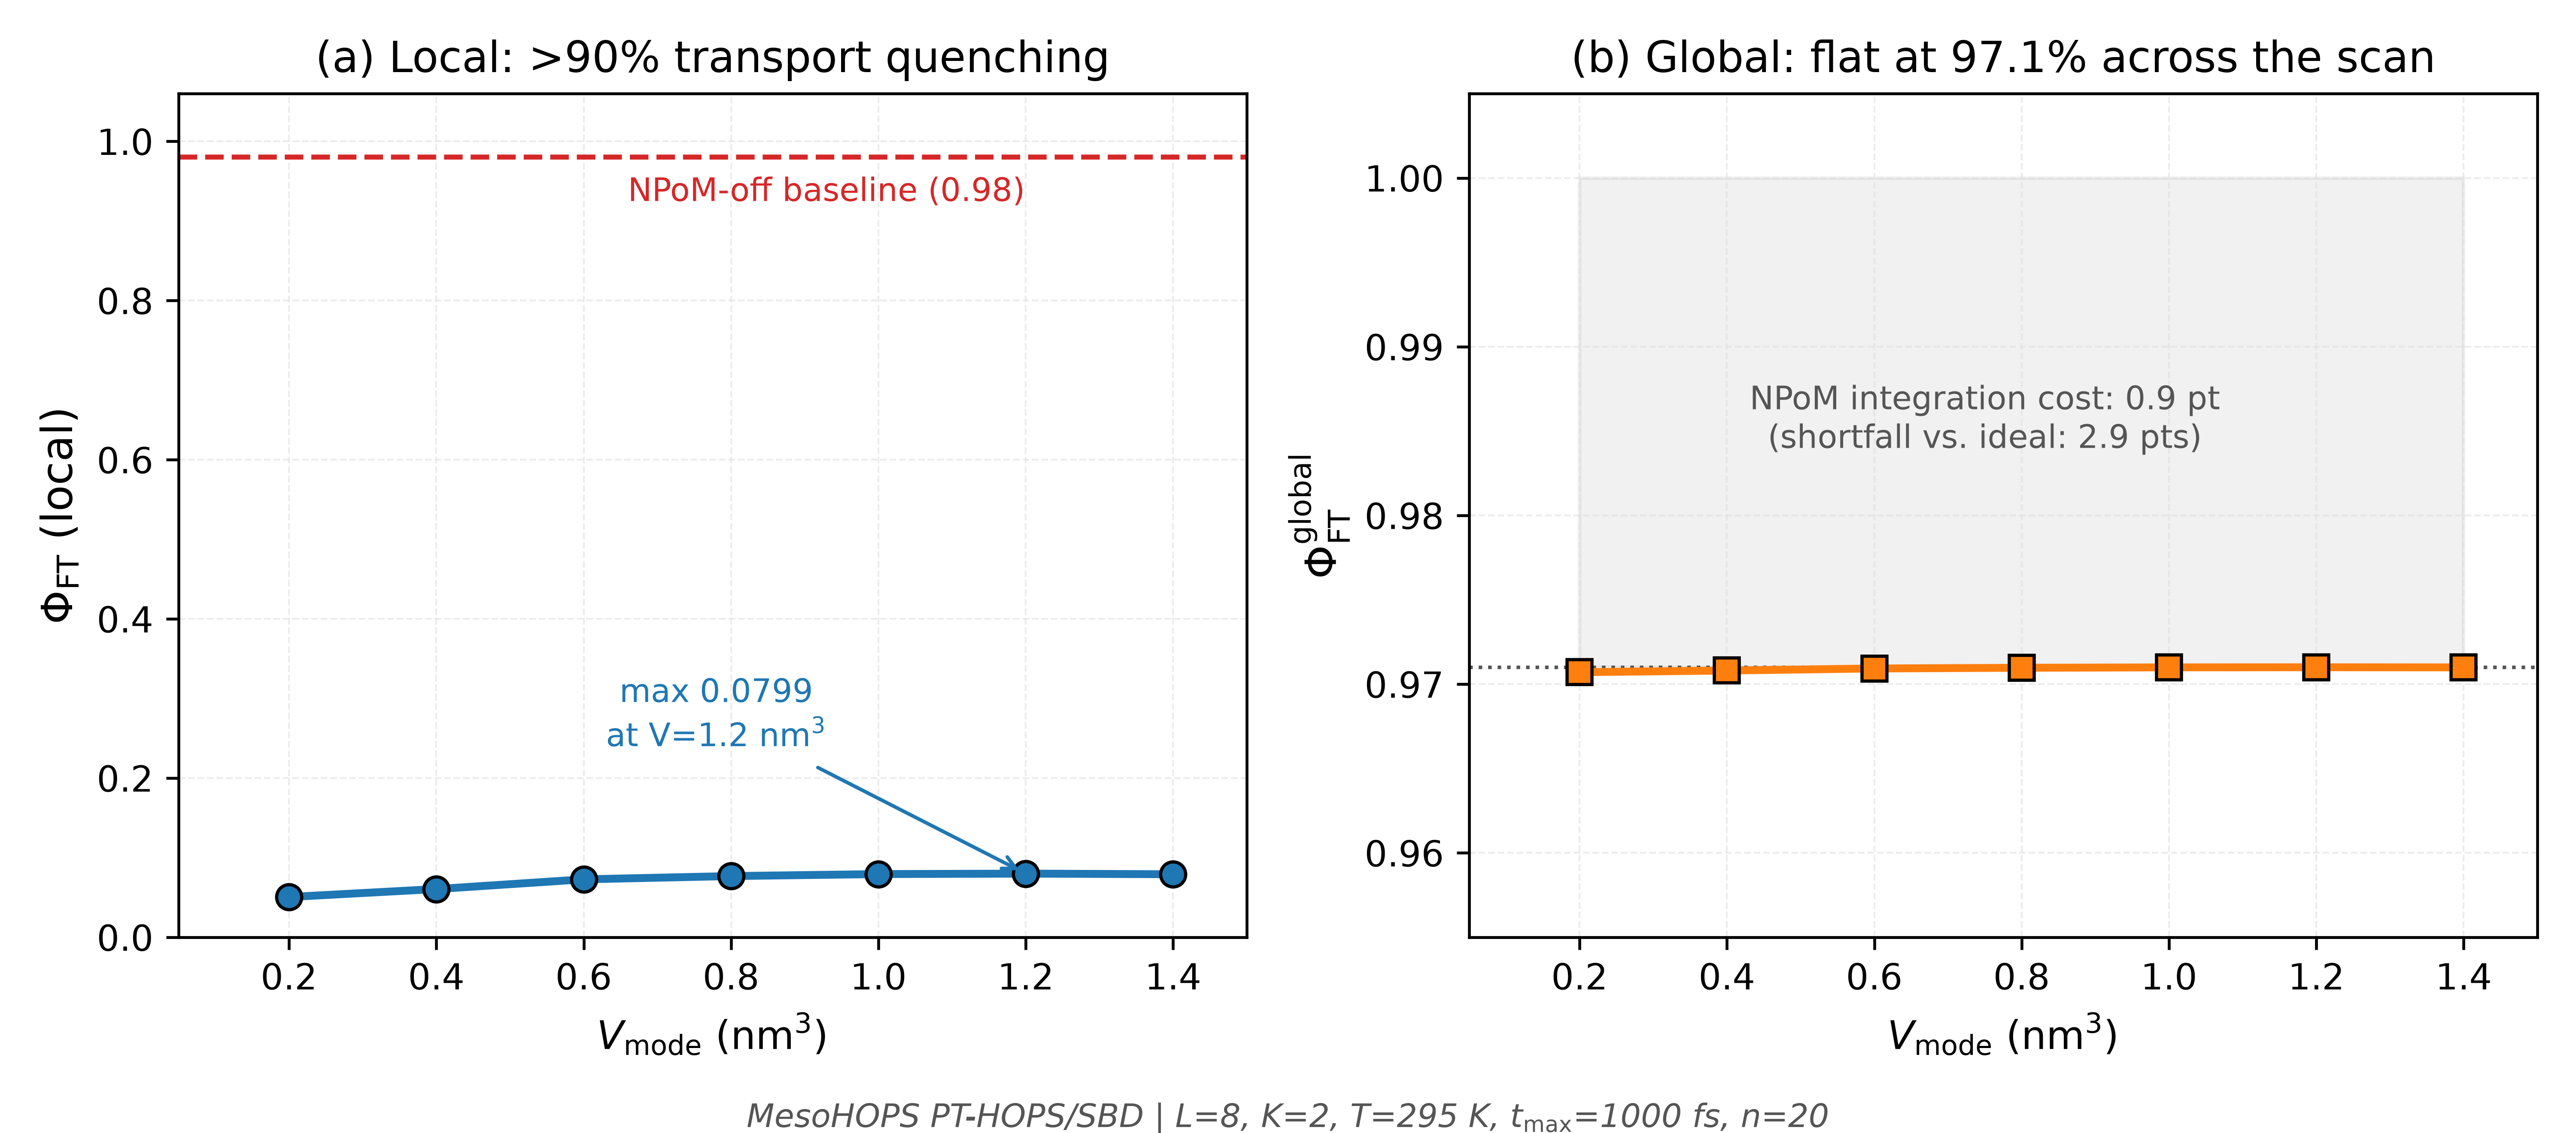
\includegraphics[width=\columnwidth]{Figure_Plateau_Canopy.png}
\caption{\textbf{Local quenching, global stability: the central result in one picture.} (a) Forward transfer yield $\Phi_{\mathrm{FT}}$ across the NPoM mode-volume scan ($n=20$, $T=\qty{295}{\K}$): locally, transport is quenched by more than \qty{90}{\percent} relative to the pristine FMO baseline ($0.98$), with a factor-1.6 variation across the accessible range and a maximum of $0.0799$ at $V_{\mathrm{mode}}=\qty{1.2}{\nm\cubed}$ (\Cref{tab:npom_volume_scan}). (b) Area-weighted global canopy trapping yield for the \qty{1}{\percent} sentinel fraction (\Cref{eq:phi_global}): flat at $\num{0.971}$ across the entire scan --- the deep local suppression is absorbed at a constant 0.9-point canopy-scale cost (\num{0.980} to \num{0.971}), leaving the canopy 2.9 points below an ideal yield of 1.0. The flat curve in (b), not the quenching in (a), is the design-relevant outcome: diagnostics integrate into the stack without compromising productivity. Provenance: the curves are plotted from the independent $n=20$ re-simulation of all seven mode volumes; the tabulated values in \Cref{tab:npom_volume_scan} are the original production runs ($n=2$ except where noted) and the re-simulation reproduces them within $\pm 0.002$.}
\label{fig:flat_canopy}
\end{figure}

\begin{figure}[htbp]
\centering
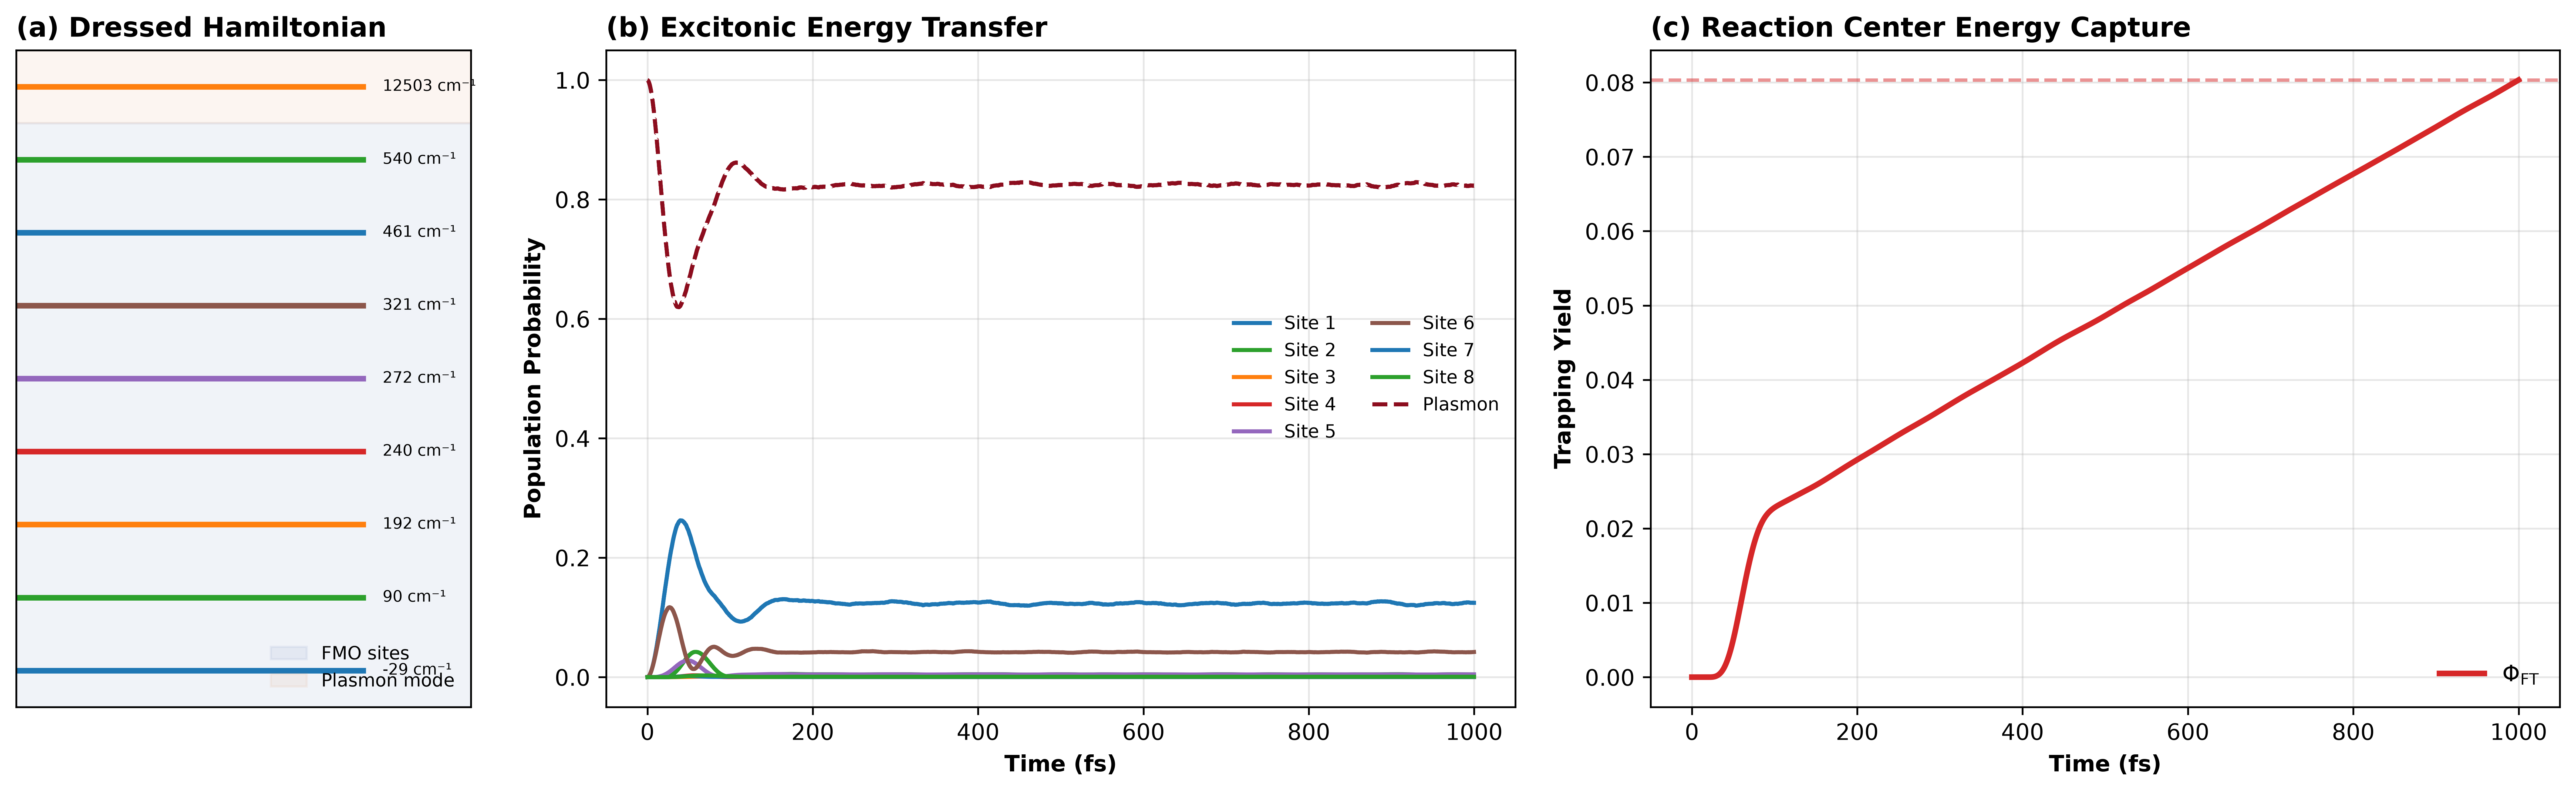
\includegraphics[width=\columnwidth]{Figure1_Quantum_Dynamics.png}
\caption{\textbf{Quantum dynamics of the 8-site FMO complex coupled to an NPoM plasmonic cavity within the agrivoltaic digital twin.}
\textbf{(a)} Energy level diagram of the $9\times 9$ dressed Hamiltonian showing the 8 FMO excitonic states coupling to the plasmon mode with strength $g_0$.
\textbf{(b)} Population dynamics of the $n=20$ production run at $V_{\mathrm{mode}} = \qty{1.2}{\nm\cubed}$ and \qty{295}{\kelvin} (the scan optimum of \Cref{tab:npom_volume_scan}): the plasmon mode (Site~9) loads within the first \qty{10}{\fs} and captures \qty{83}{\percent} of the excitation, starving the trapping sites --- the microscopic origin of the \qty{91.8}{\percent} local penalty.
\textbf{(c)} Cumulative reaction-center trapping yield $\Phi_{\mathrm{FT}}(t)$ for the same run, saturating at \num{0.0799}.
All data: $L=8$, $K=2$, $n=20$ disorder realizations (\Cref{SI-sec:comparative_hdf5}). The passive-fraction dynamics underlying the coherence and yield gains of \Cref{fig:quantum_dynamics}c are reported in~\cite{TeguiaKouam2026}. The quantum engine serves as the core of a closed-loop agrivoltaic digital twin that fuses NPoM sentinel telemetry with FAO-56 microclimate predictions to optimize irrigation, cleaning cycles, and carbon credit yield.}
\label{fig:quantum_dynamics}
\end{figure}

\begin{figure}[htbp]
\centering
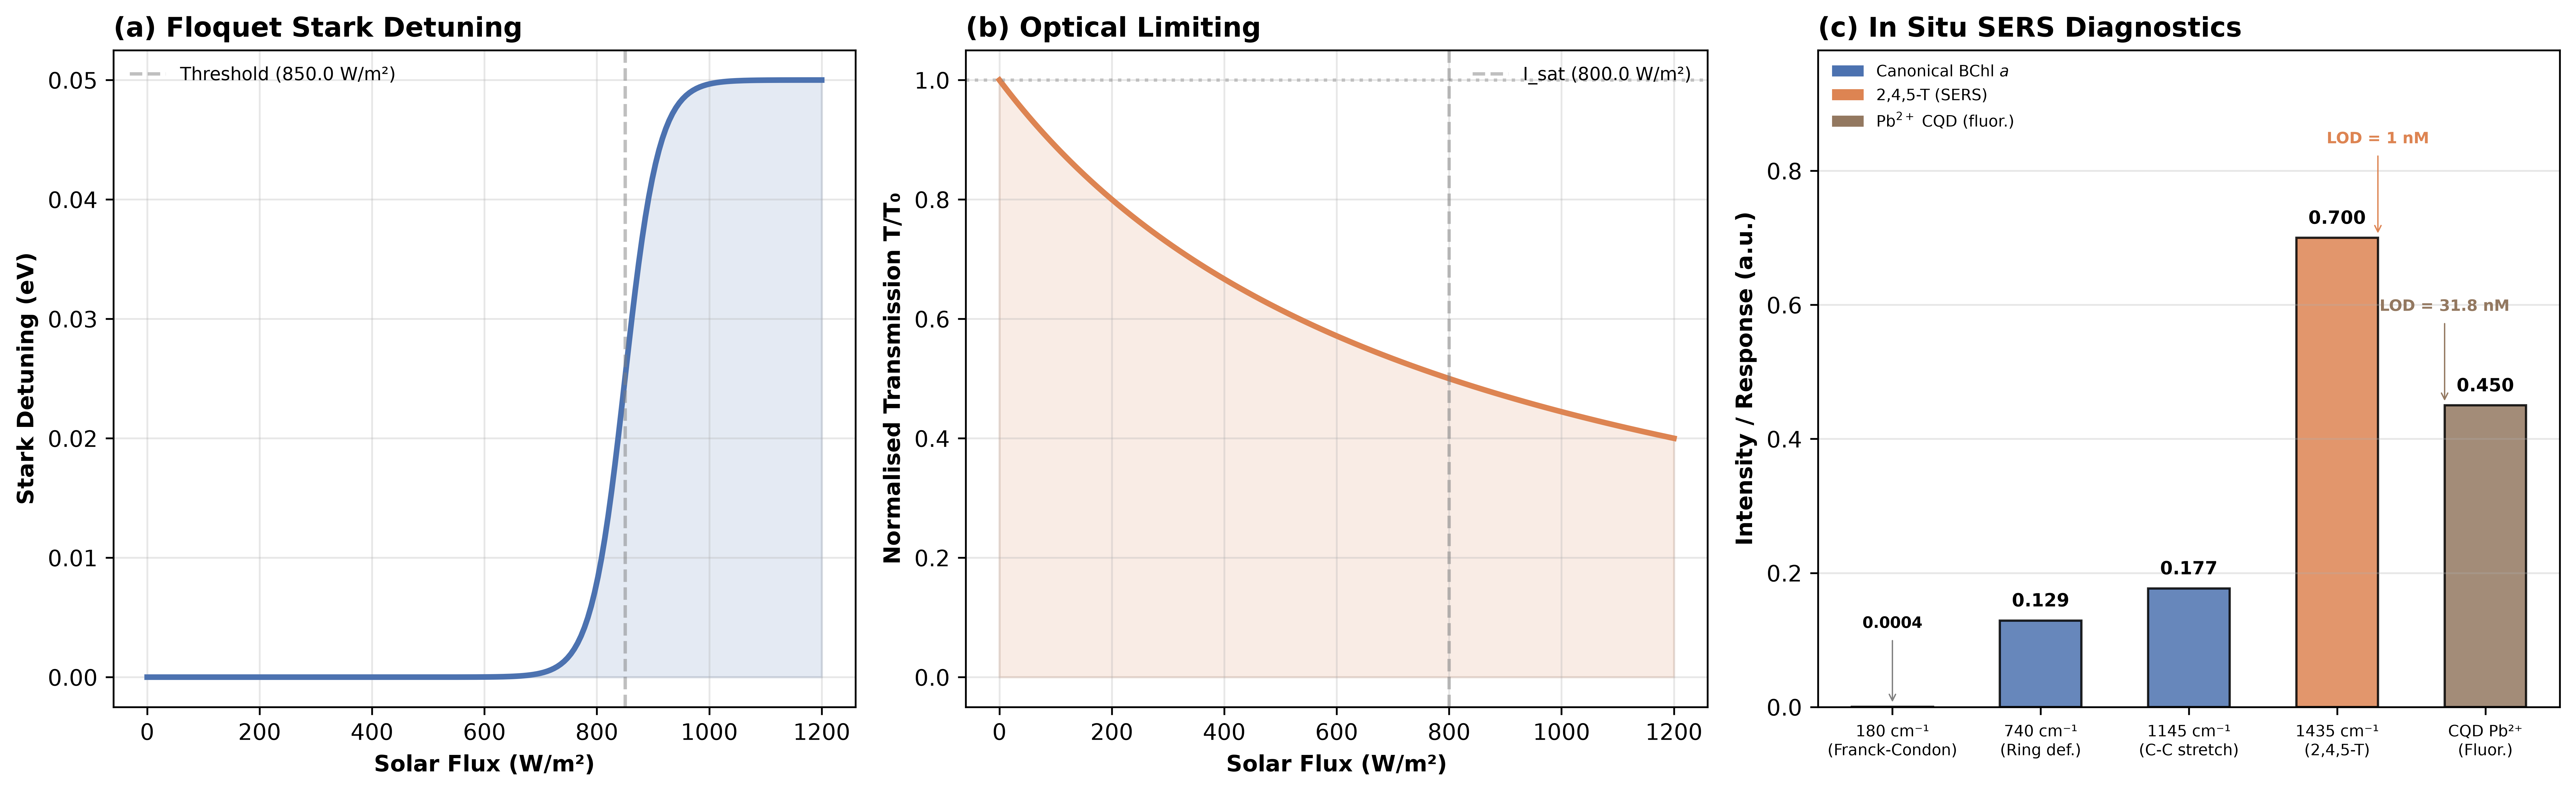
\includegraphics[width=\columnwidth]{Figure2_SERS_Readout.png}
\caption{\textbf{Dynamic photo-protection, in situ diagnostics, and environmental robustness.}
\textbf{(a)} Floquet Stark detuning amplitude as a function of solar flux: the hysteretic switch closes the resonant site-1 and site-6 transfer channels when the flux rises above \qty{850}{\W\per\m\squared} and reopens only below \qty{750}{\W\per\m\squared} ($\Delta = \qty{403}{\per\cm} \gg |J_{12}| = \qty{87.7}{\per\cm}$, single-channel transmission $\sim$0.05) --- the solid-state analogue of non-photochemical quenching.
\textbf{(b)} Flux-dependent optical limiting of the \qty{750}{\nm} and \qty{820}{\nm} passbands: at \qty{1000}{\W\per\m\squared} the two filter passbands themselves close to \qty{44}{\percent} of baseline, protecting the exciton budget precisely where the co-designed filter concentrates it.
\textbf{(c)} Simulated SERS Raman spectrum showing the canonical BChl $a$ vibrational modes (\qty{180}{\per\cm}, \qty{740}{\per\cm}, \qty{1145}{\per\cm}). The three agriculturally specific target signatures assigned to the sentinel sub-system --- oxidative stress (\qty{1145}{\per\cm}), 2,4,5-T pesticide contamination (\qty{1435}{\per\cm}, LOD = \qty{1}{\nano\mol\per\L}), and \ce{Pb^{2+}} via encapsulated \ce{CdTe/ZnSe} quantum dot fluorescence quenching (LOD = \qty{31.8}{\nano\mol\per\L}) --- are detailed in the main text and SI. A DynamicCalibrator using exponential moving average ($\alpha = 0.1$) of daily reference readings corrects sensor baseline drift from biofouling, raising an alarm when drift exceeds \qty{20}{\percent} of the initial baseline.}
\label{fig:npq_switch}
\end{figure}

\begin{figure}[htbp]
\centering
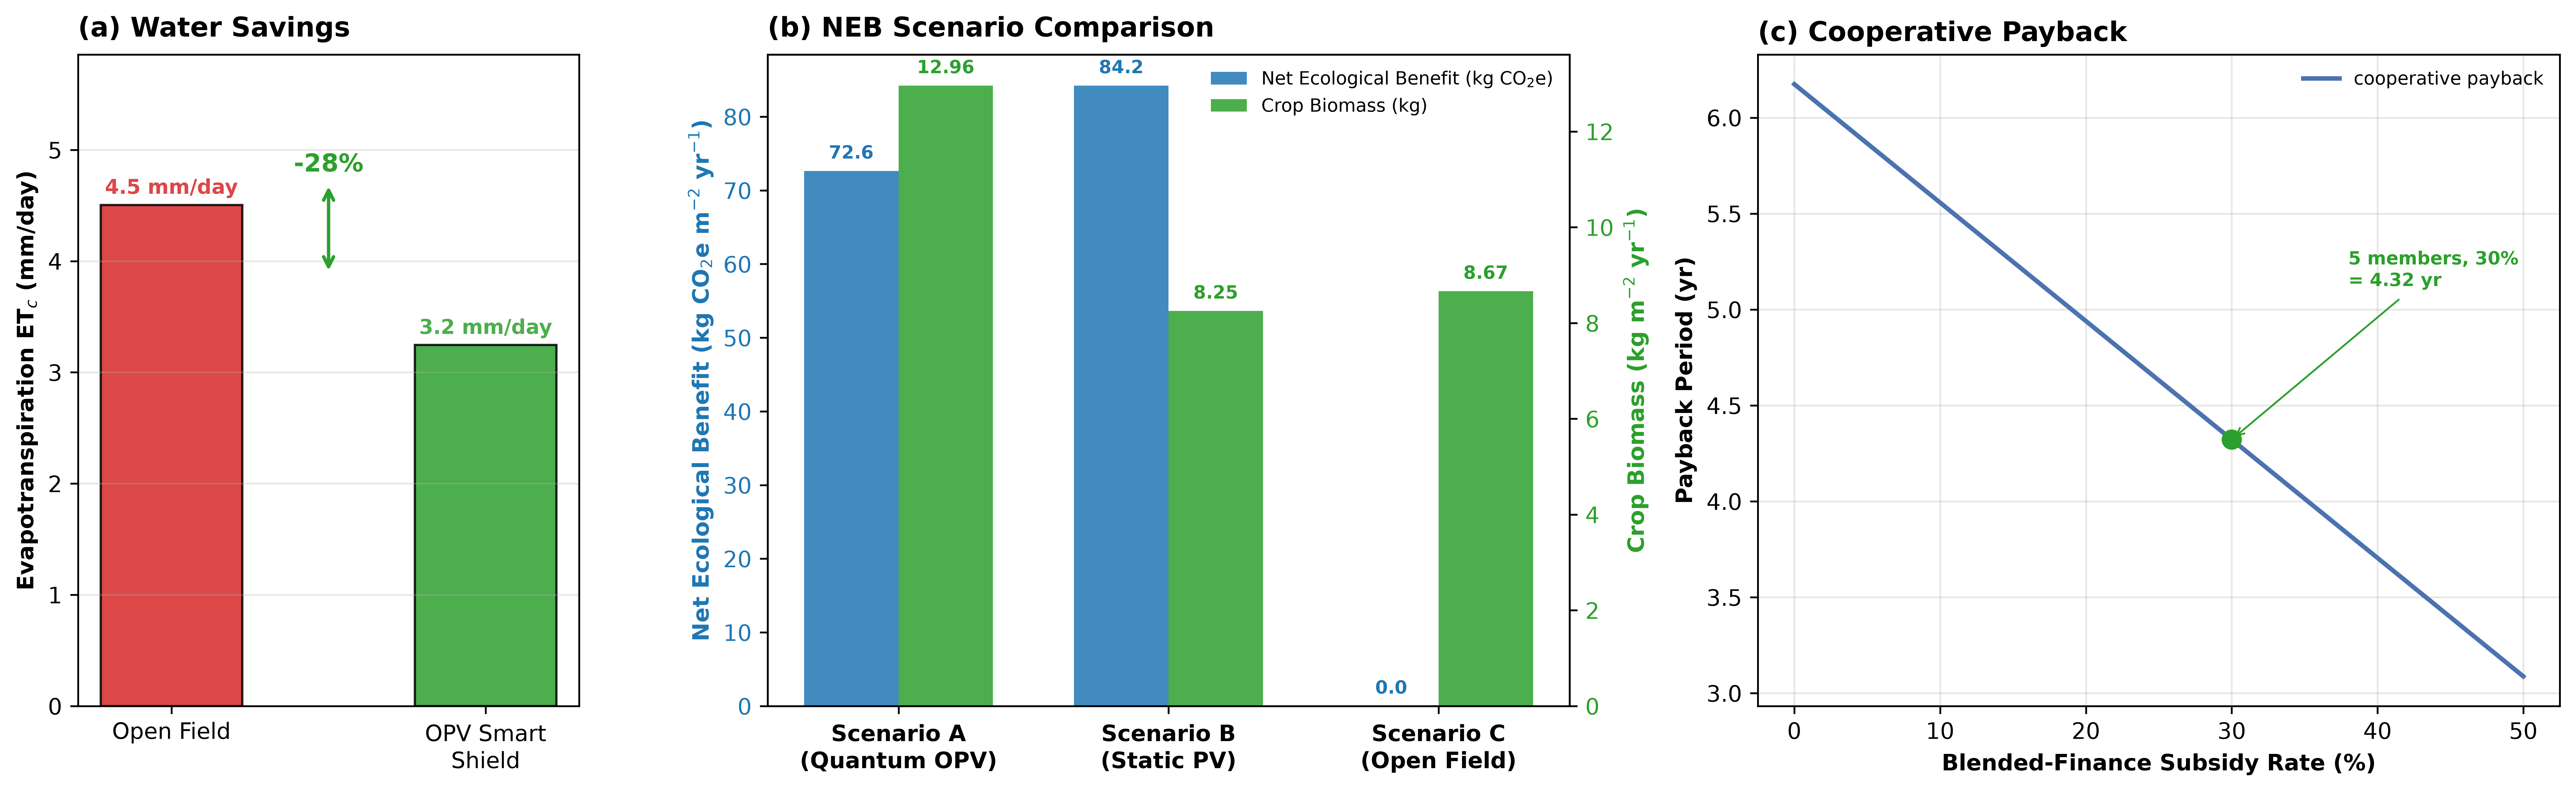
\includegraphics[width=\columnwidth]{Figure3_LCA_NEB_Comparison.png}
\caption{\textbf{Water--Energy--Food network assessment.} All panels refer to the \qty{500}{\m\squared} high-tunnel floriculture micro-module in Cameroon's Western Highlands described in \Cref{sec:methods_poc}.
\textbf{(a)} FAO-56 evapotranspiration comparison: open field ($\mathrm{ET}_c = \qty{4.5}{\mm\per\day}$) vs.\ OPV smart shield ($\mathrm{ET}_c = \qty{3.2}{\mm\per\day}$), a \qty{28}{\percent} reduction.
\textbf{(b)} Net Ecological Benefit comparison across three operating scenarios: Quantum OPV (A: OPV--NPoM shield with dual-band transmission and the quantum-fertilizer biomass boost), Static shading (B: opaque static-shading module --- higher PV output, suppressed canopy), and Open field (C: no module). Scenario A achieves \qty{72.6}{\kg\of{\ce{CO2e}}\per\m\squared\per\yr} with an effective crop biomass of \qty{13.0}{\kg\per\m\squared\per\yr}, while Scenario B reaches \qty{84.2}{\kg\of{\ce{CO2e}}\per\m\squared\per\yr} but only \qty{8.2}{\kg\per\m\squared\per\yr} in biomass (plotted bar values \num{12.96}, \num{8.25} and \num{8.67}, rounded in the text). The comparison is deliberately uncomfortable: an opaque static module still buys more carbon than the quantum shield, but it does so by suppressing the canopy to \qty{84}{\percent} of reference biomass, whereas the quantum shield preserves near-baseline productivity (\num{0.971} global trapping yield, \num{13.0} including biostimulation) --- exactly the food--energy trade-off that motivates spectral co-design. The NEB serves as the verifiable metric for a tiered subsidy framework that bridges the quantum divide.
\textbf{(c)} Simple, undiscounted payback period of the module as a function of the blended-finance subsidy rate (five-member cooperative; the discounted NPV and its discount-rate sensitivity are reported in the text and \Cref{SI-sec:socioeconomic}). At the modeled \qty{30}{\percent} subsidy, payback = \qty{4.32}{\yr} (net annual cashflow of \qty{26075}{\USD\per\yr} after OPEX). This indicates that, under the modeled cooperative assumptions, quantum-guided agrivoltaics can shorten payback when coupled with cooperative ownership and strategic crop selection.}
\label{fig:lca_comparison}
\end{figure}

\begin{figure}[htbp]
\centering
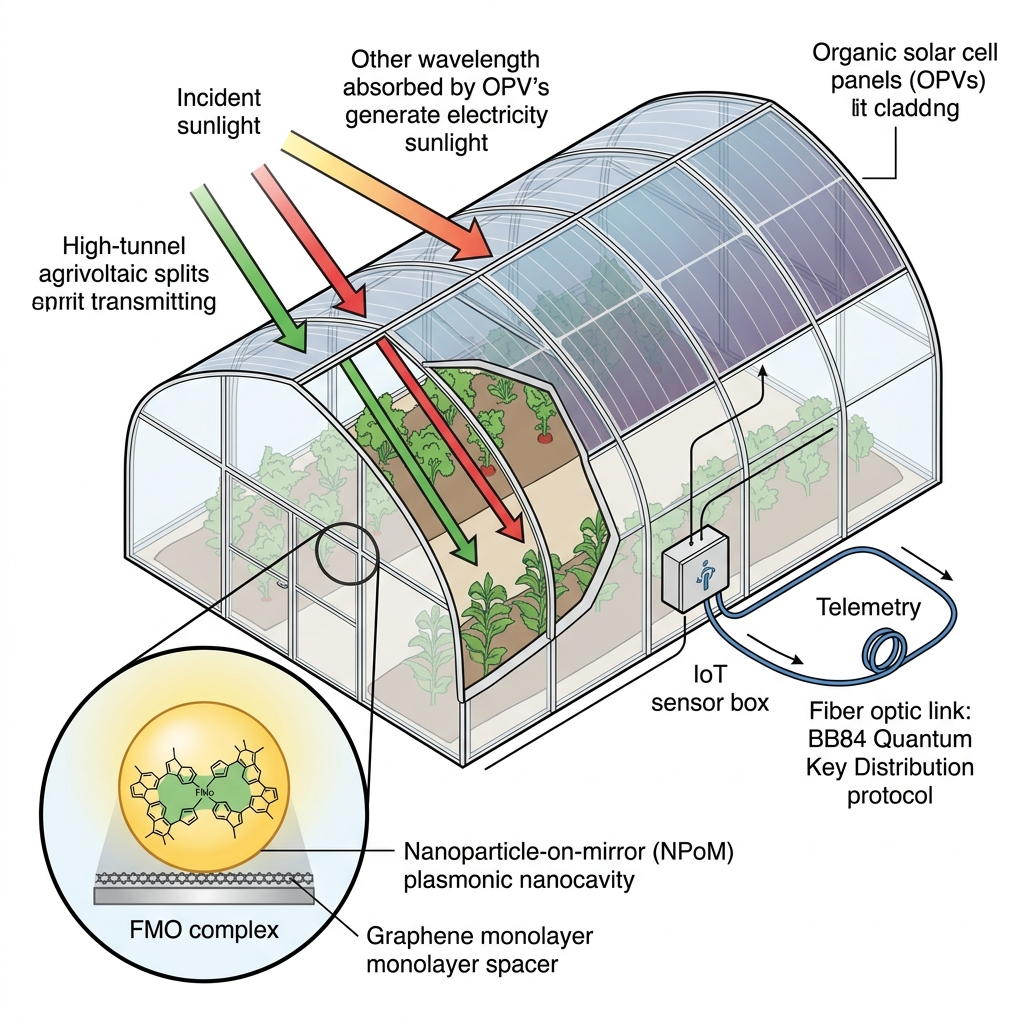
\includegraphics[width=0.63\columnwidth]{Figure_Setup_Dispositif.png}
\caption{\textbf{Schematic layout of the multi-scale quantum agrivoltaic digital twin platform.} Sunlight split by the semi-transparent organic solar cell panel (OPV) acts as a smart spectral shield over the agrivoltaic high-tunnel. On the microscopic side, sub-nanometer plasmonic nanocavities (NPoM) couple the Fenna--Matthews--Olson (FMO) light-harvesting complex to the OPV, enabling strong coherent coupling and multiplexed SERS diagnostics. Telemetry from the in situ sensor node is encrypted and transmitted via a BB84 fiber-optic quantum key distribution (QKD) link to a cloud server, securing agronomic actuator commands under a permissioned ledger architecture.}
\label{fig:system_setup}
\end{figure}

% =============================================================================
% REFERENCES
% =============================================================================

\bibliographystyle{elsarticle-num}
\bibliography{references}

\end{document}
